\documentclass{beamer}
\usepackage{amsmath}
\usepackage{tipa}
\usepackage[utf8]{inputenc}
\usepackage{xmpmulti}

\mode<presentation>{
\definecolor{cured}{rgb}{.8,0,.2}
\usecolortheme[named=cured]{structure}
\usetheme{split}
}
 
\newcommand{\taco}{\raisebox{-.1ex}{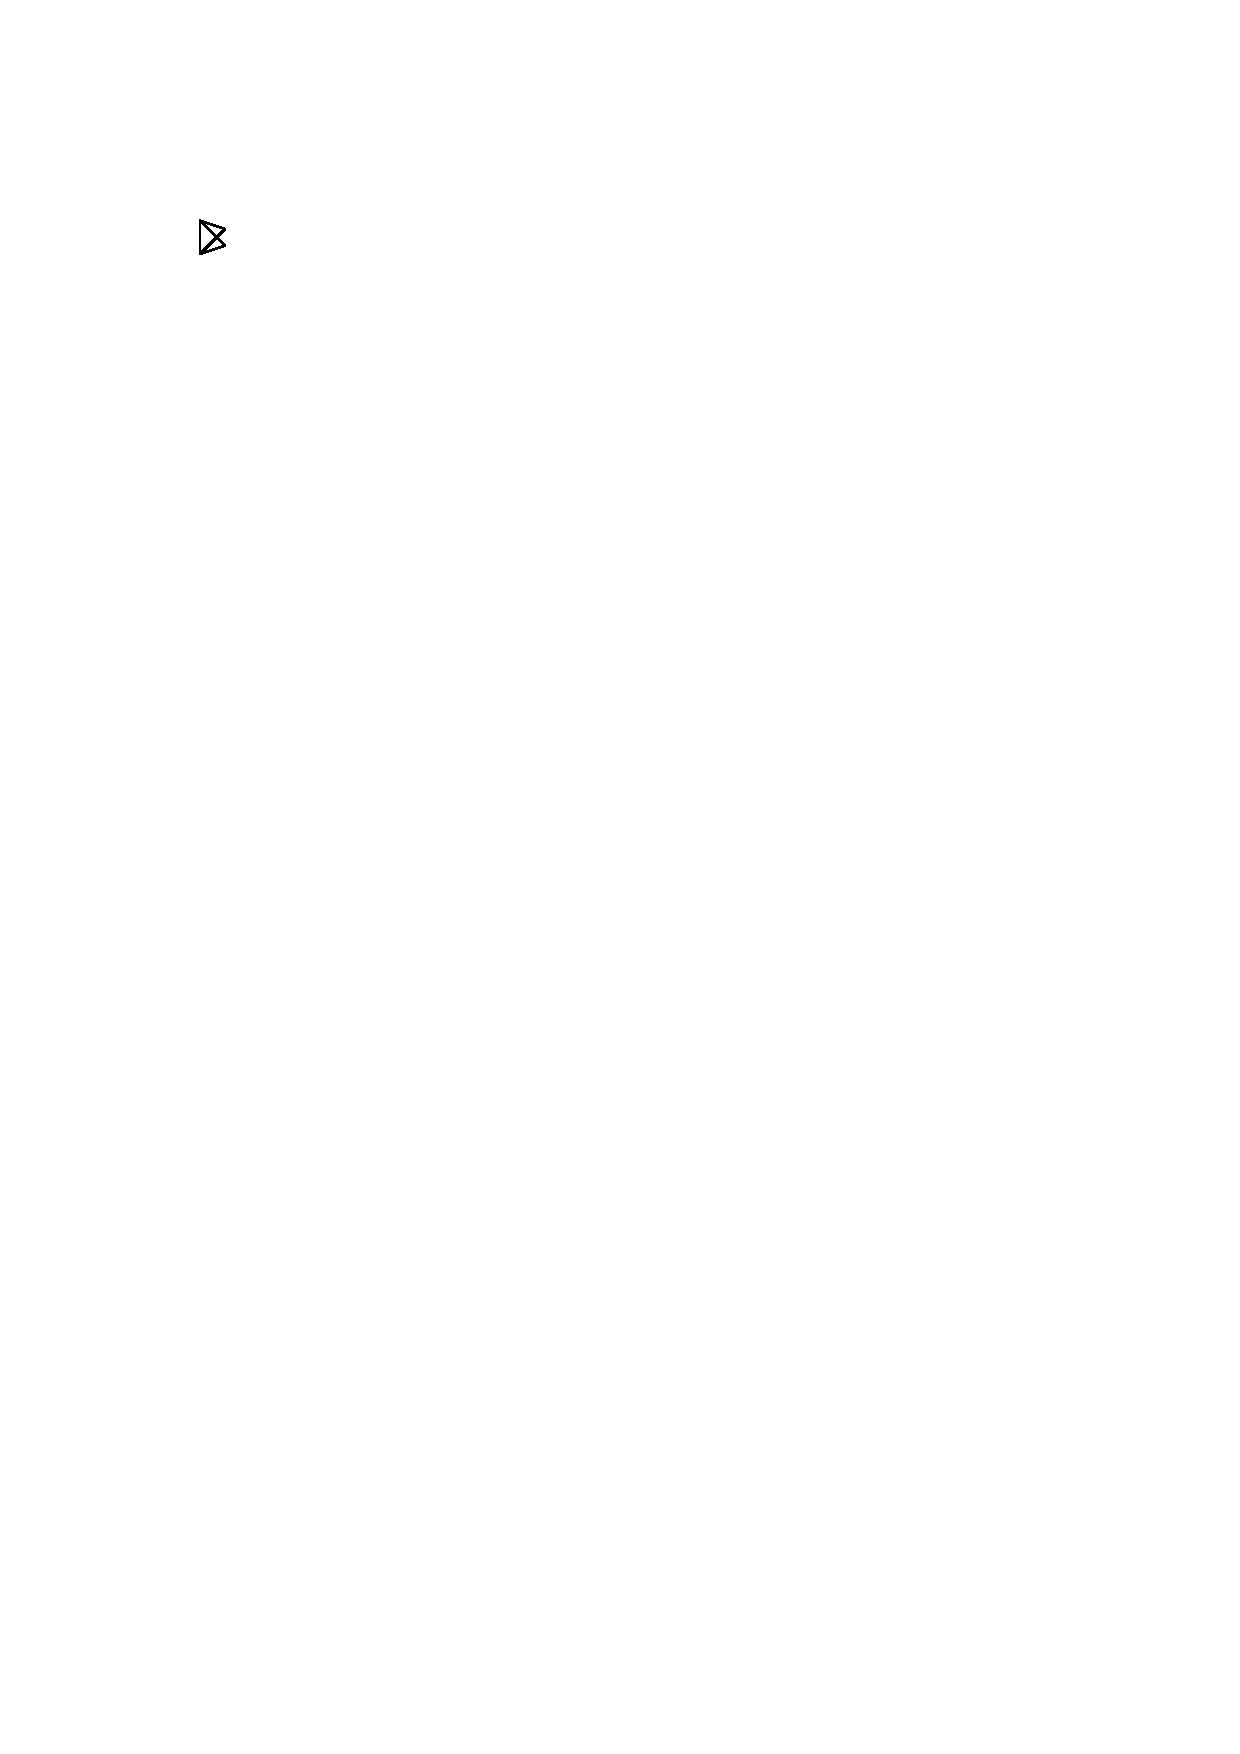
\includegraphics[height=2.0ex]{figs/triangles-edge-1}}}
\newcommand{\mariposa}{\raisebox{-.1ex}{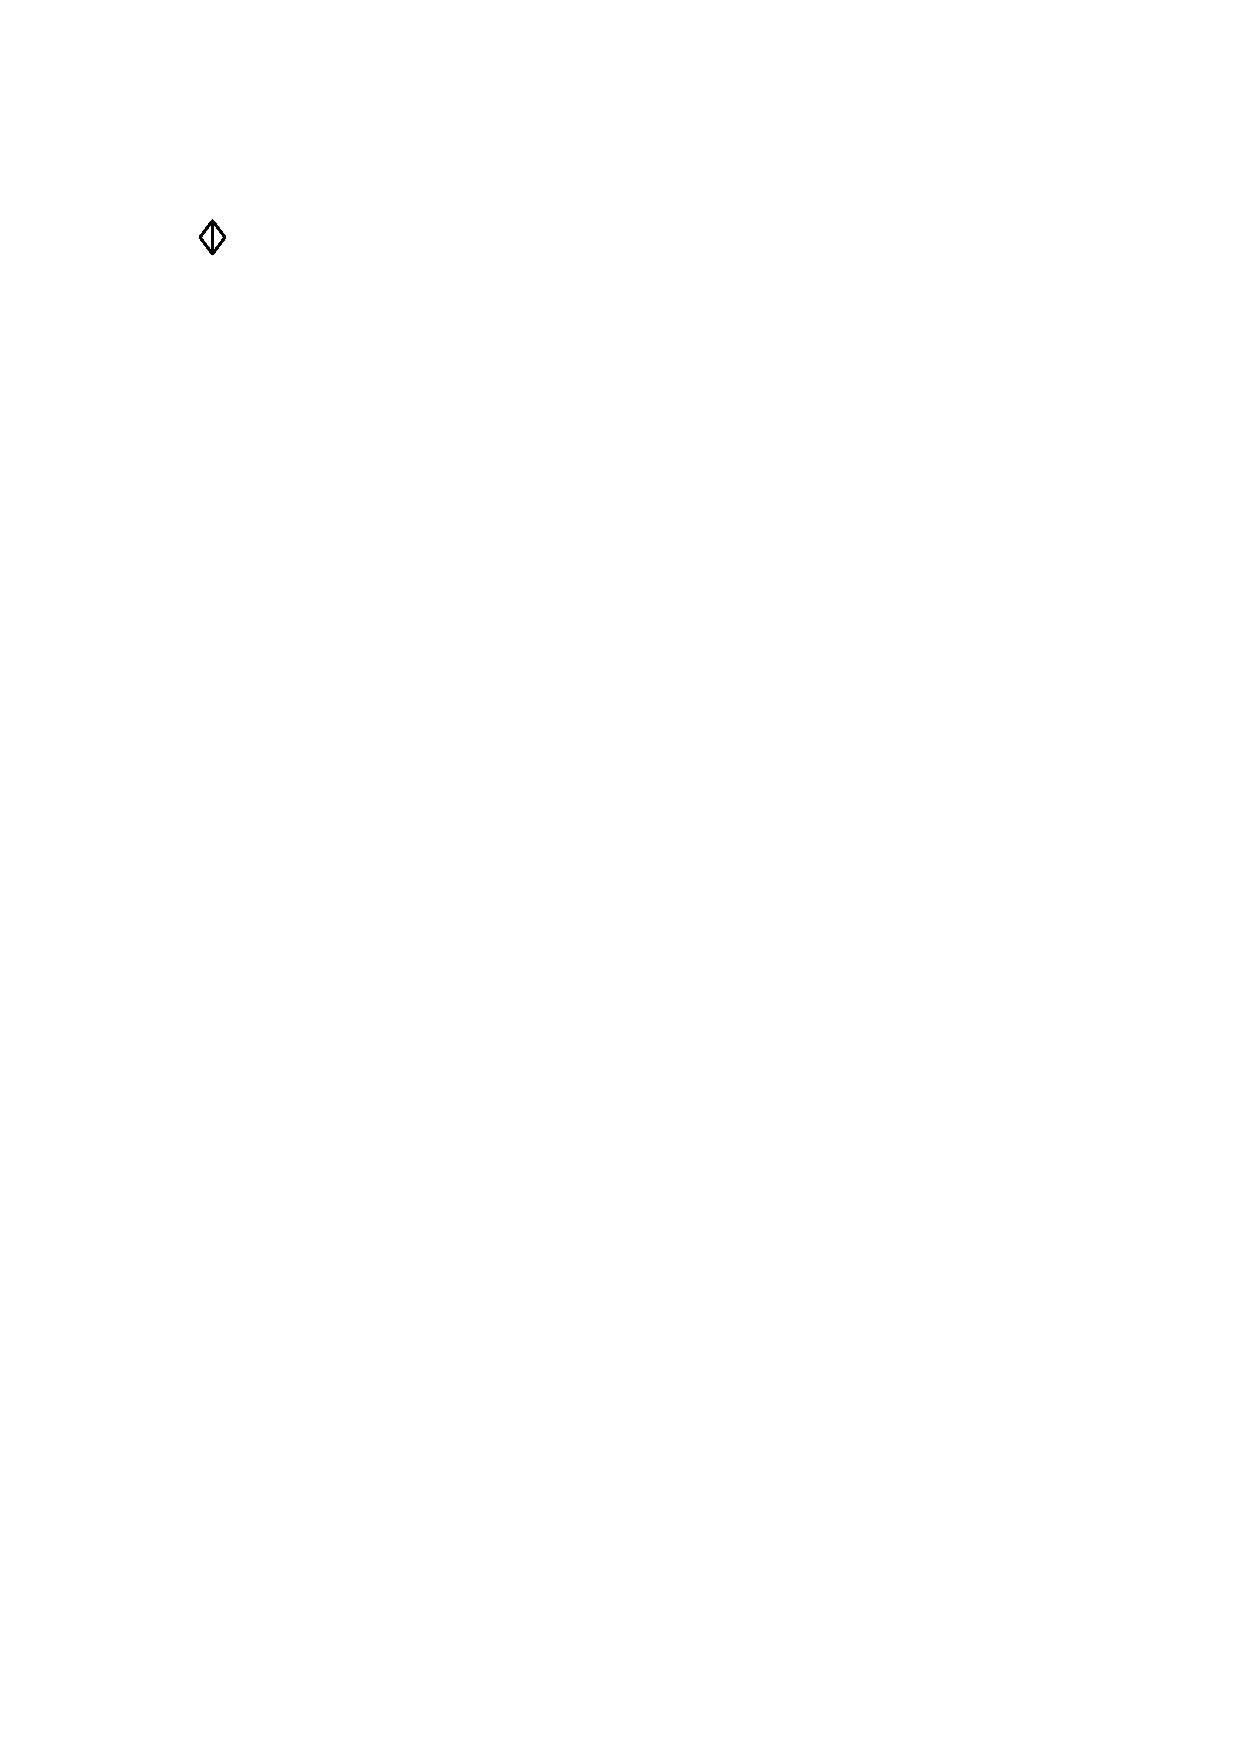
\includegraphics[height=2.0ex]{figs/triangles-edge-2}}}


\newcommand{\bat}{\raisebox{-.1ex}{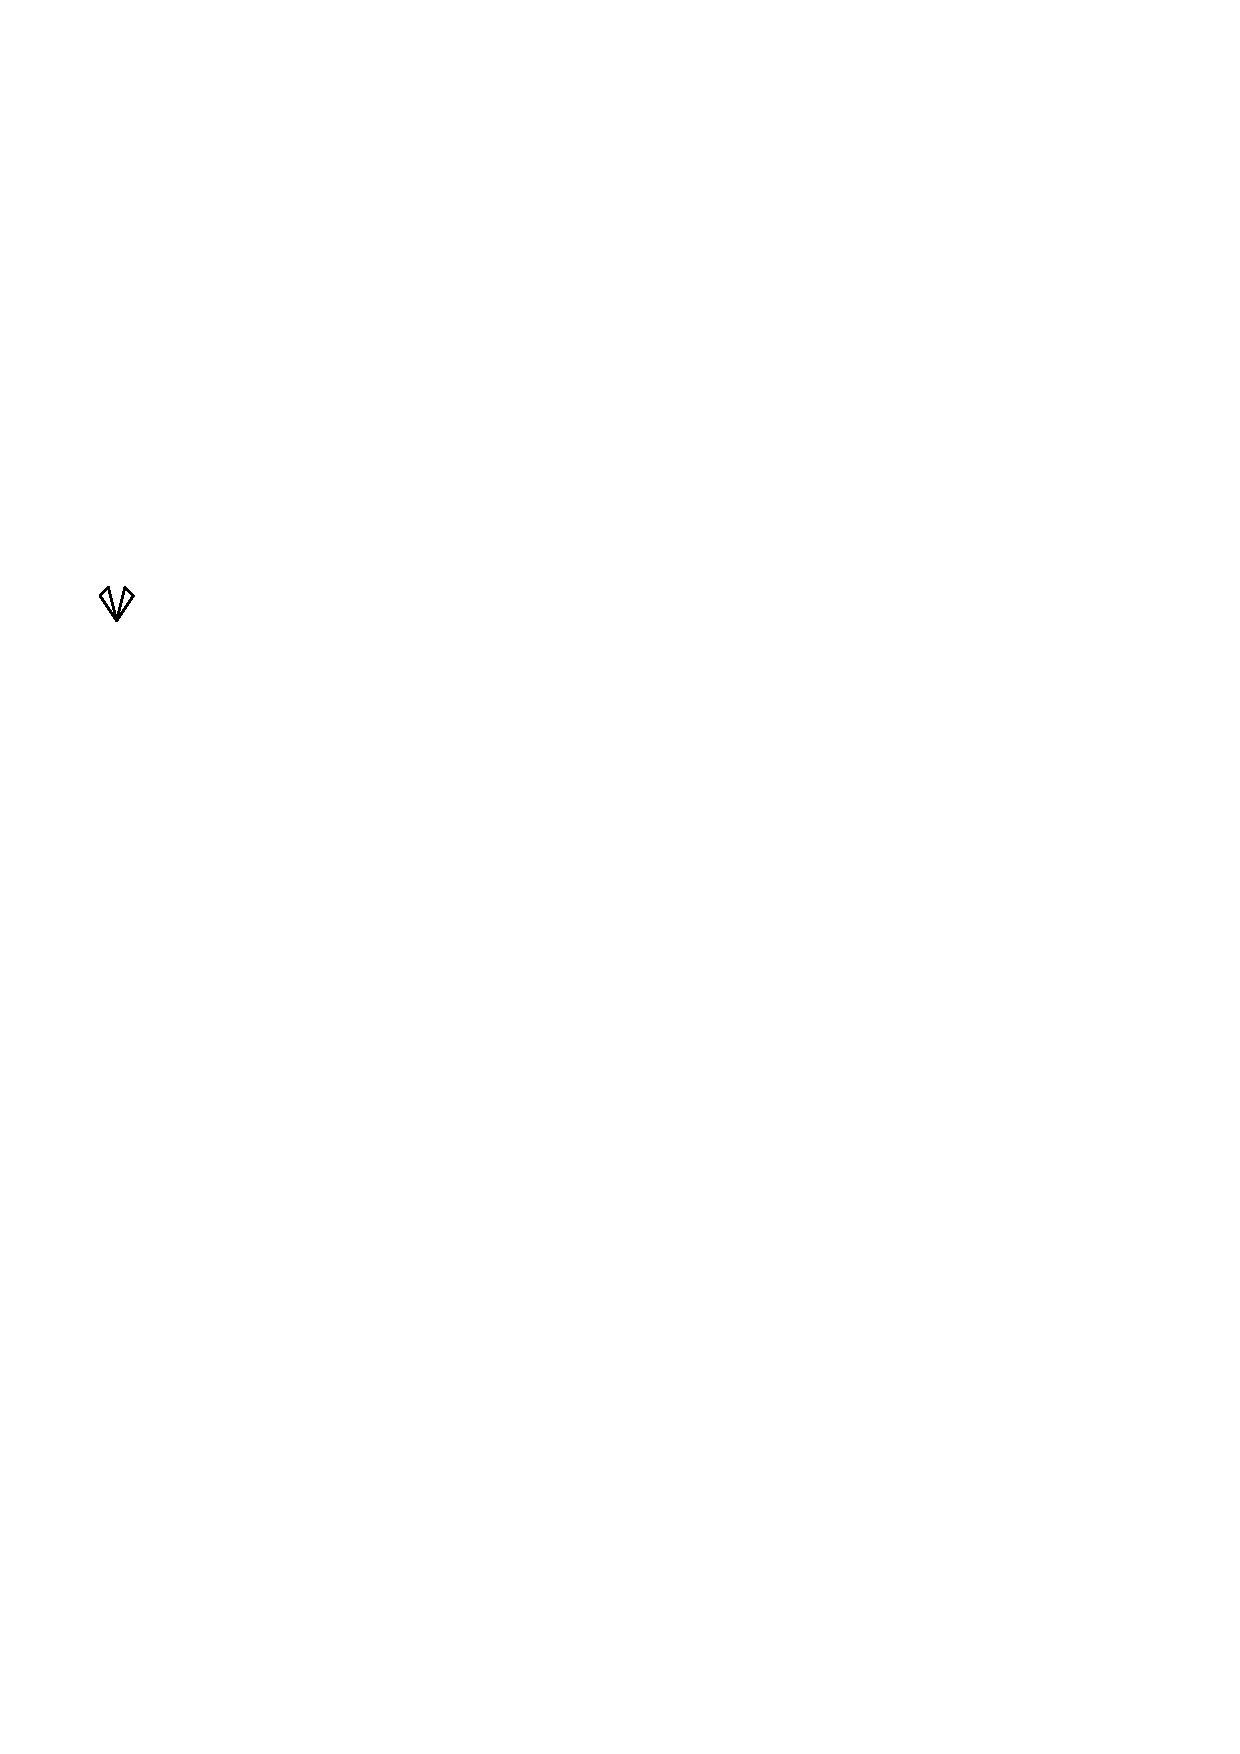
\includegraphics[height=2.0ex]{figs/triangles-vertex-1}}}
\newcommand{\nested}{\raisebox{-.1ex}{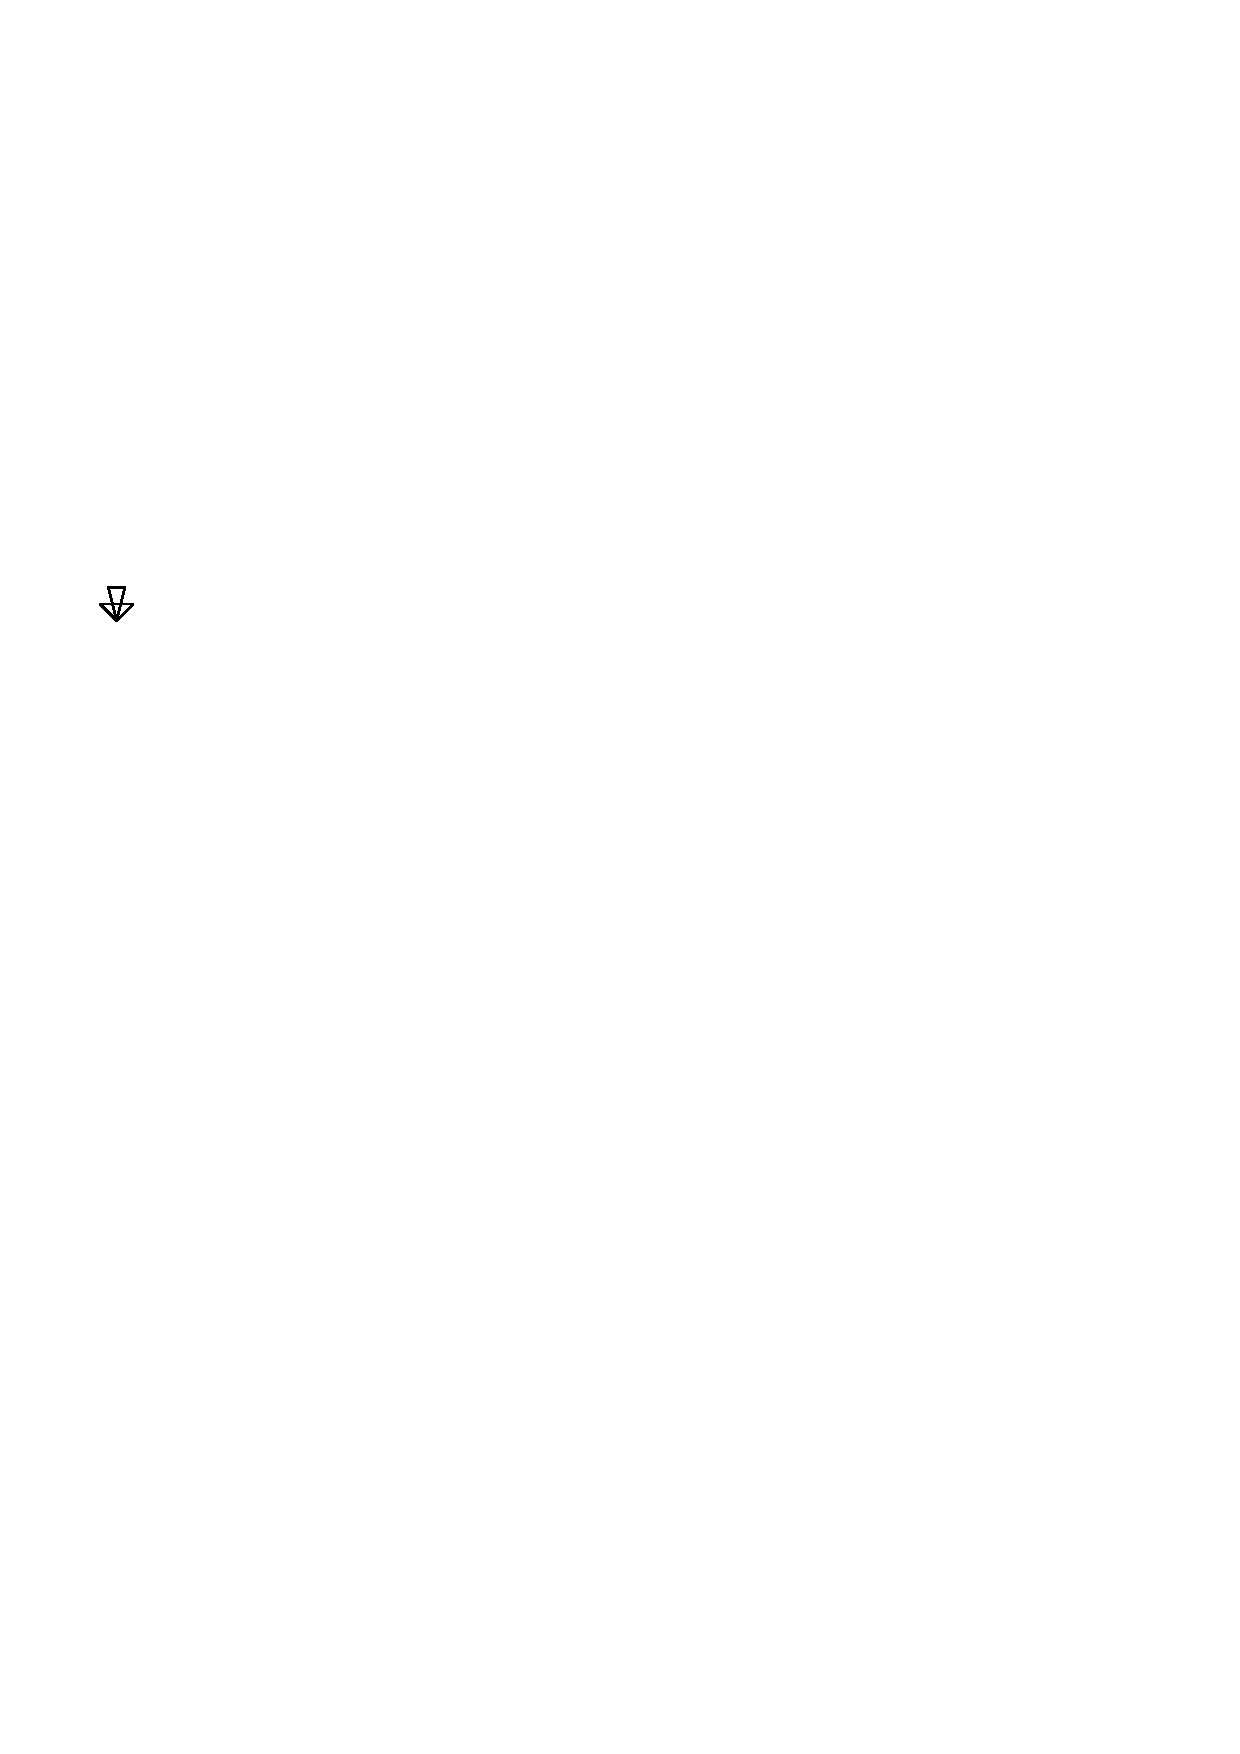
\includegraphics[height=2.0ex]{figs/triangles-vertex-2}}}
\newcommand{\crossing}{\raisebox{-.1ex}{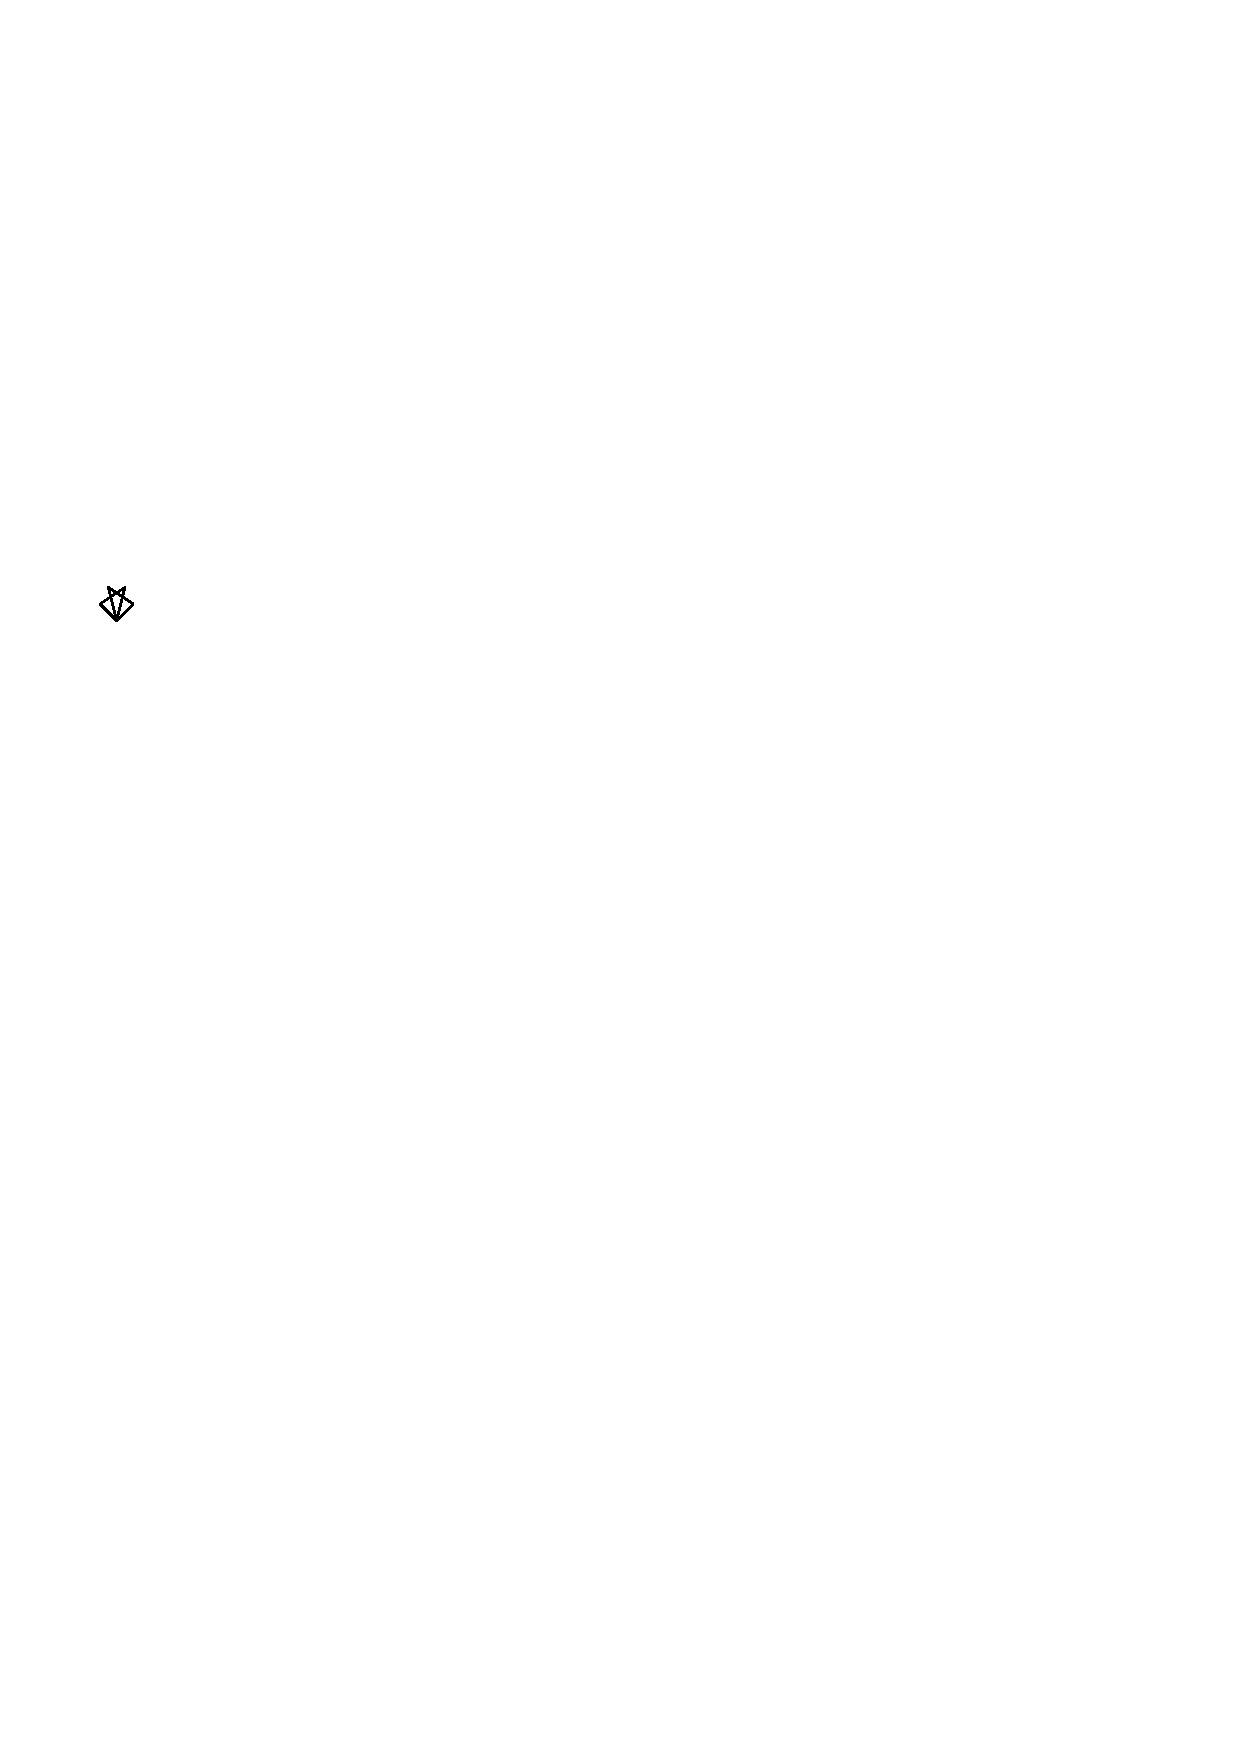
\includegraphics[height=2.0ex]{figs/triangles-vertex-3}}}

\newcommand{\ears}{\raisebox{-.1ex}{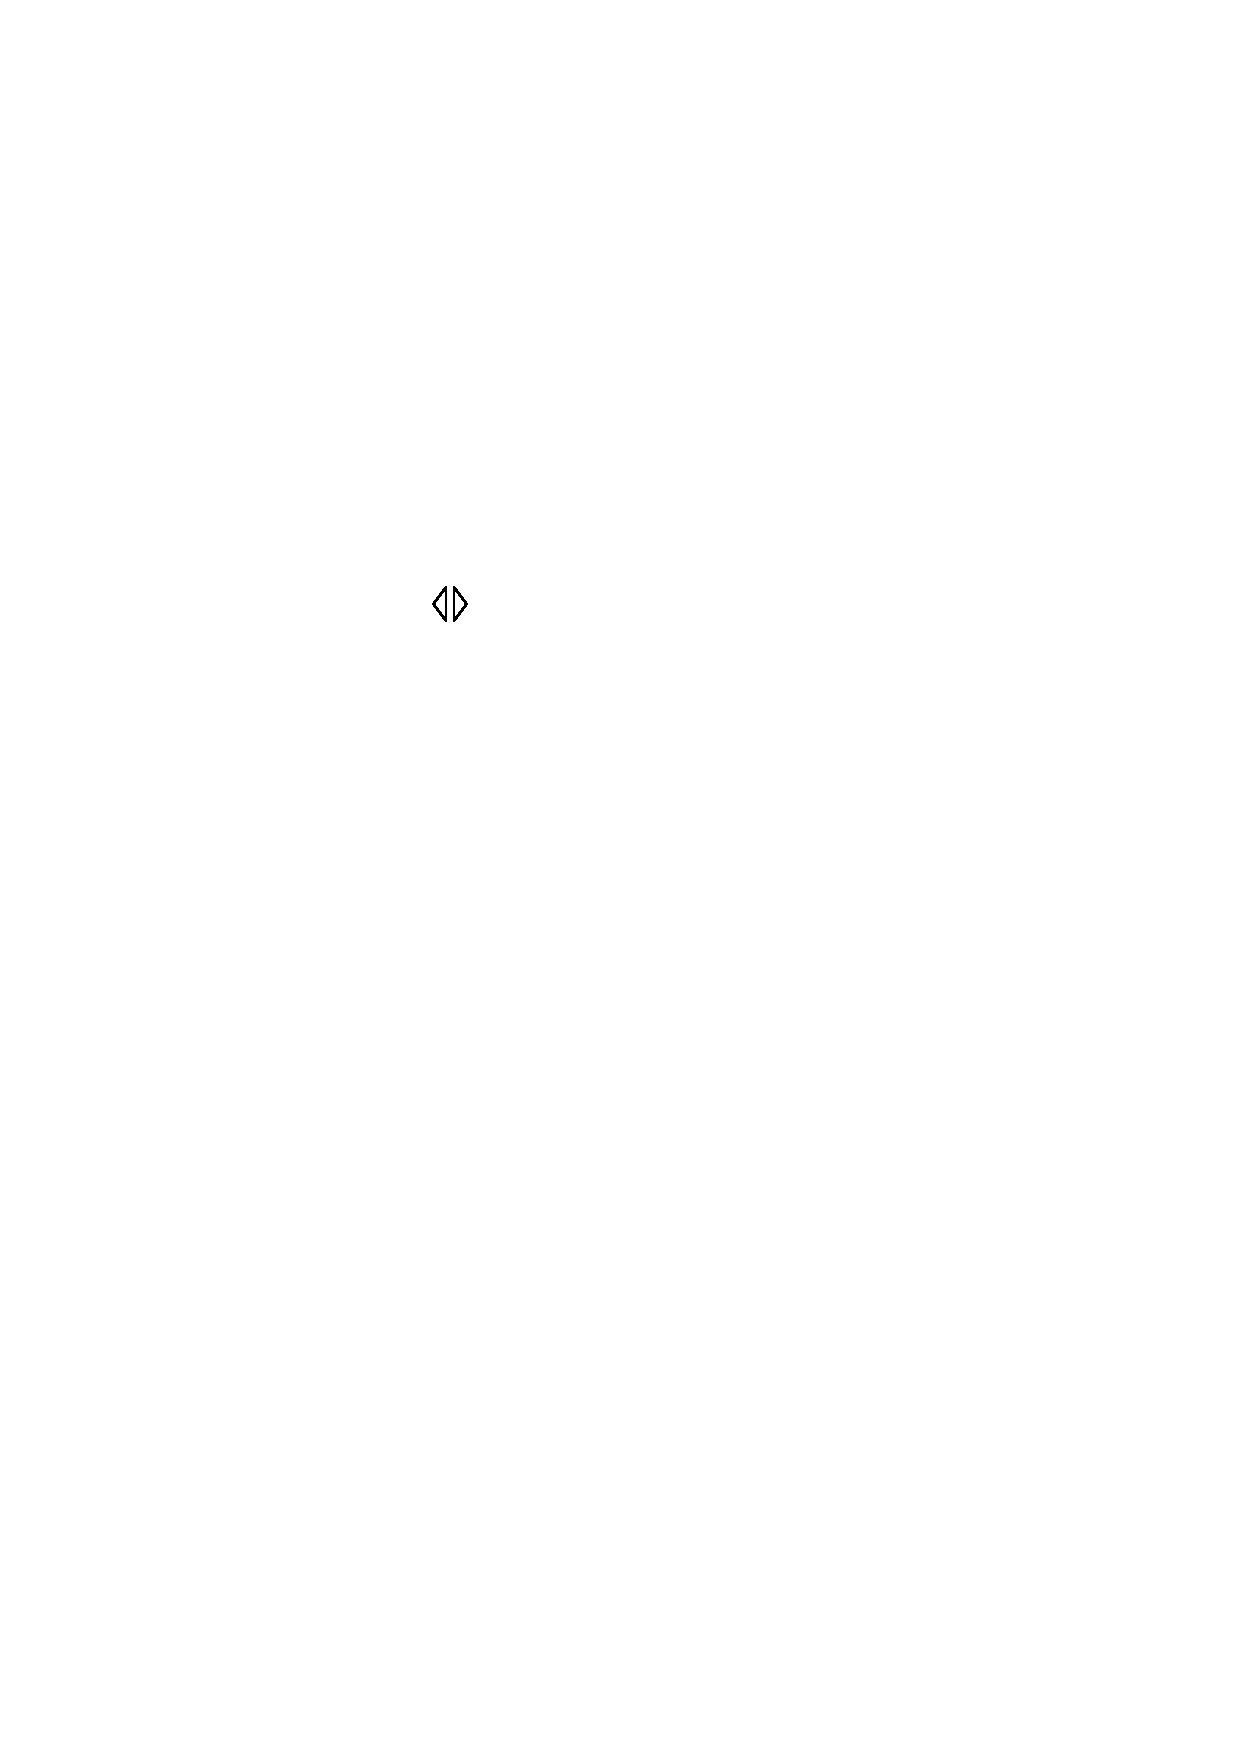
\includegraphics[height=2.0ex]{figs/triangles-disjoint-1}}}
\newcommand{\swords}{\raisebox{-.1ex}{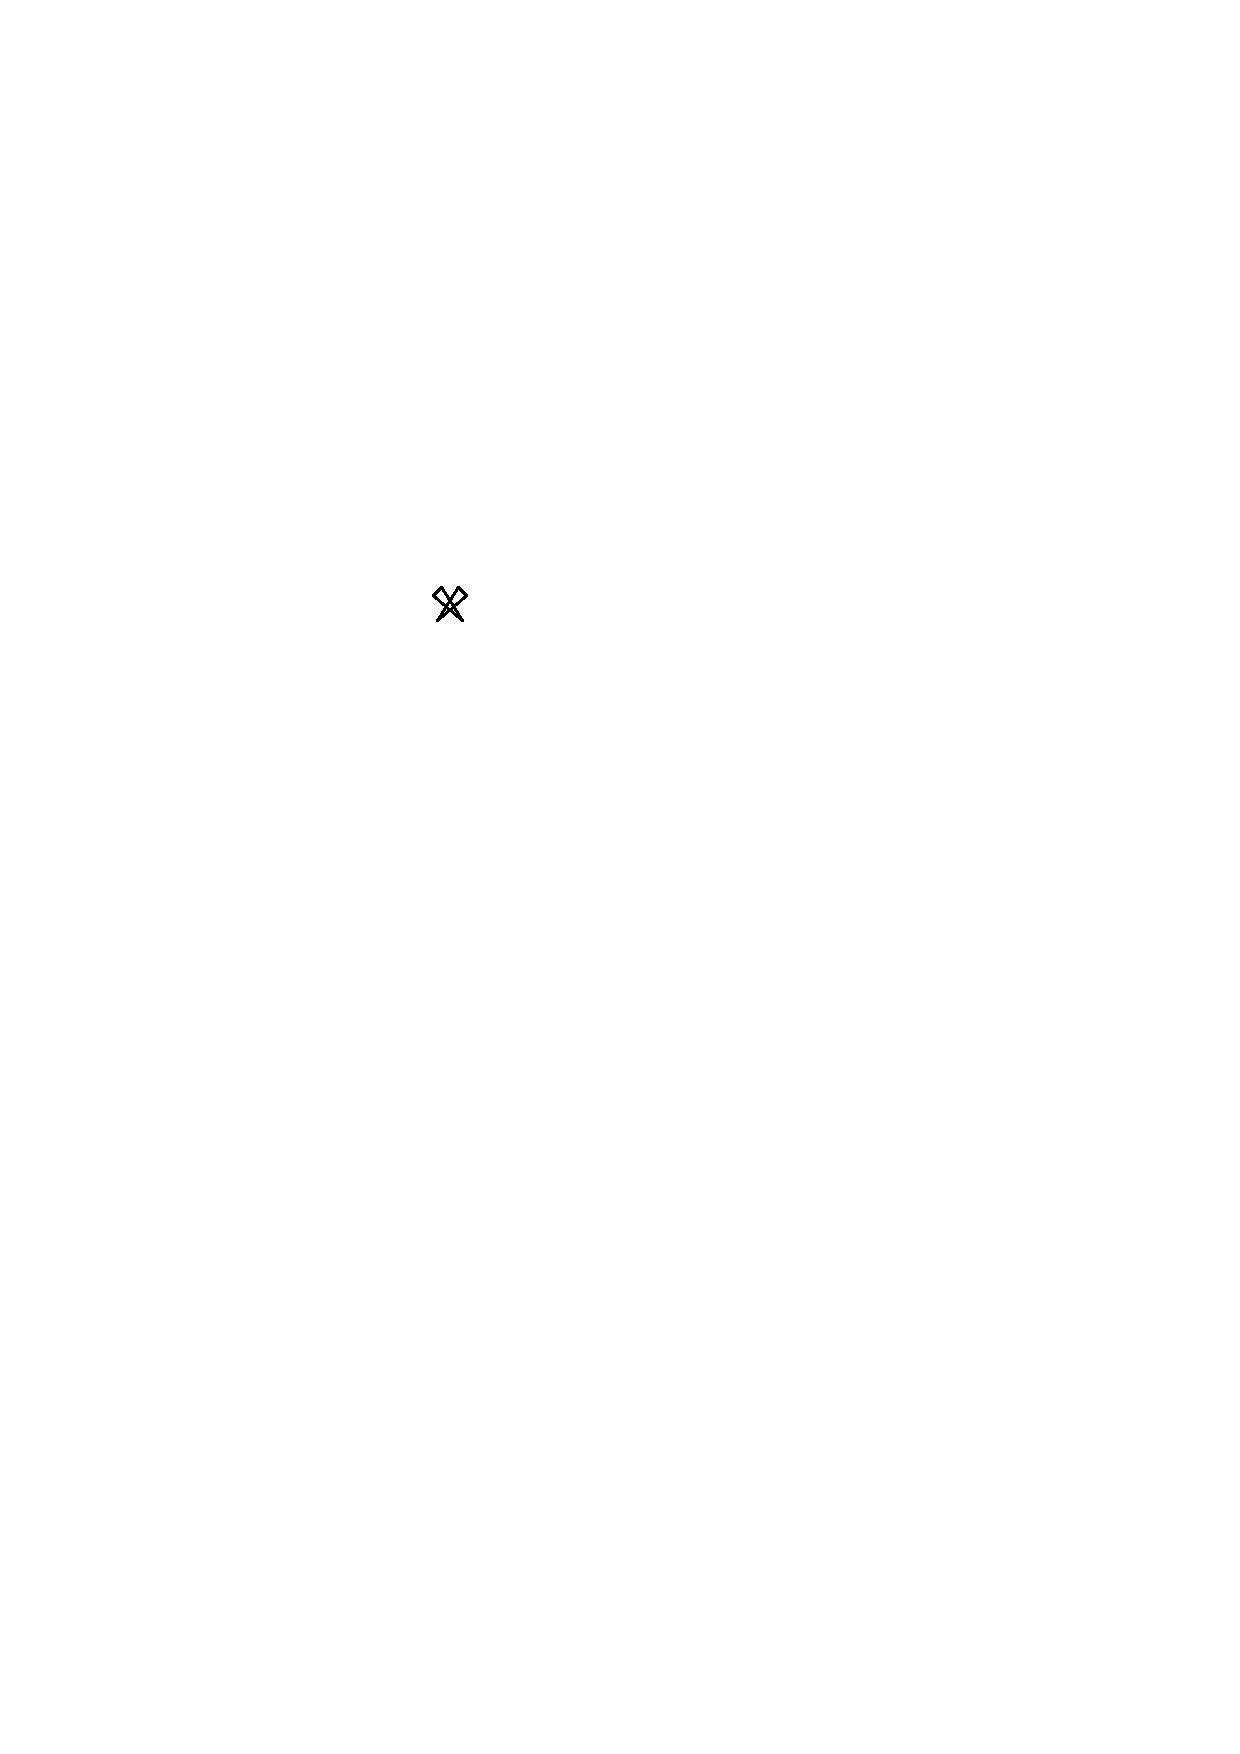
\includegraphics[height=2.0ex]{figs/triangles-disjoint-2}}}
\newcommand{\david}{\raisebox{-.1ex}{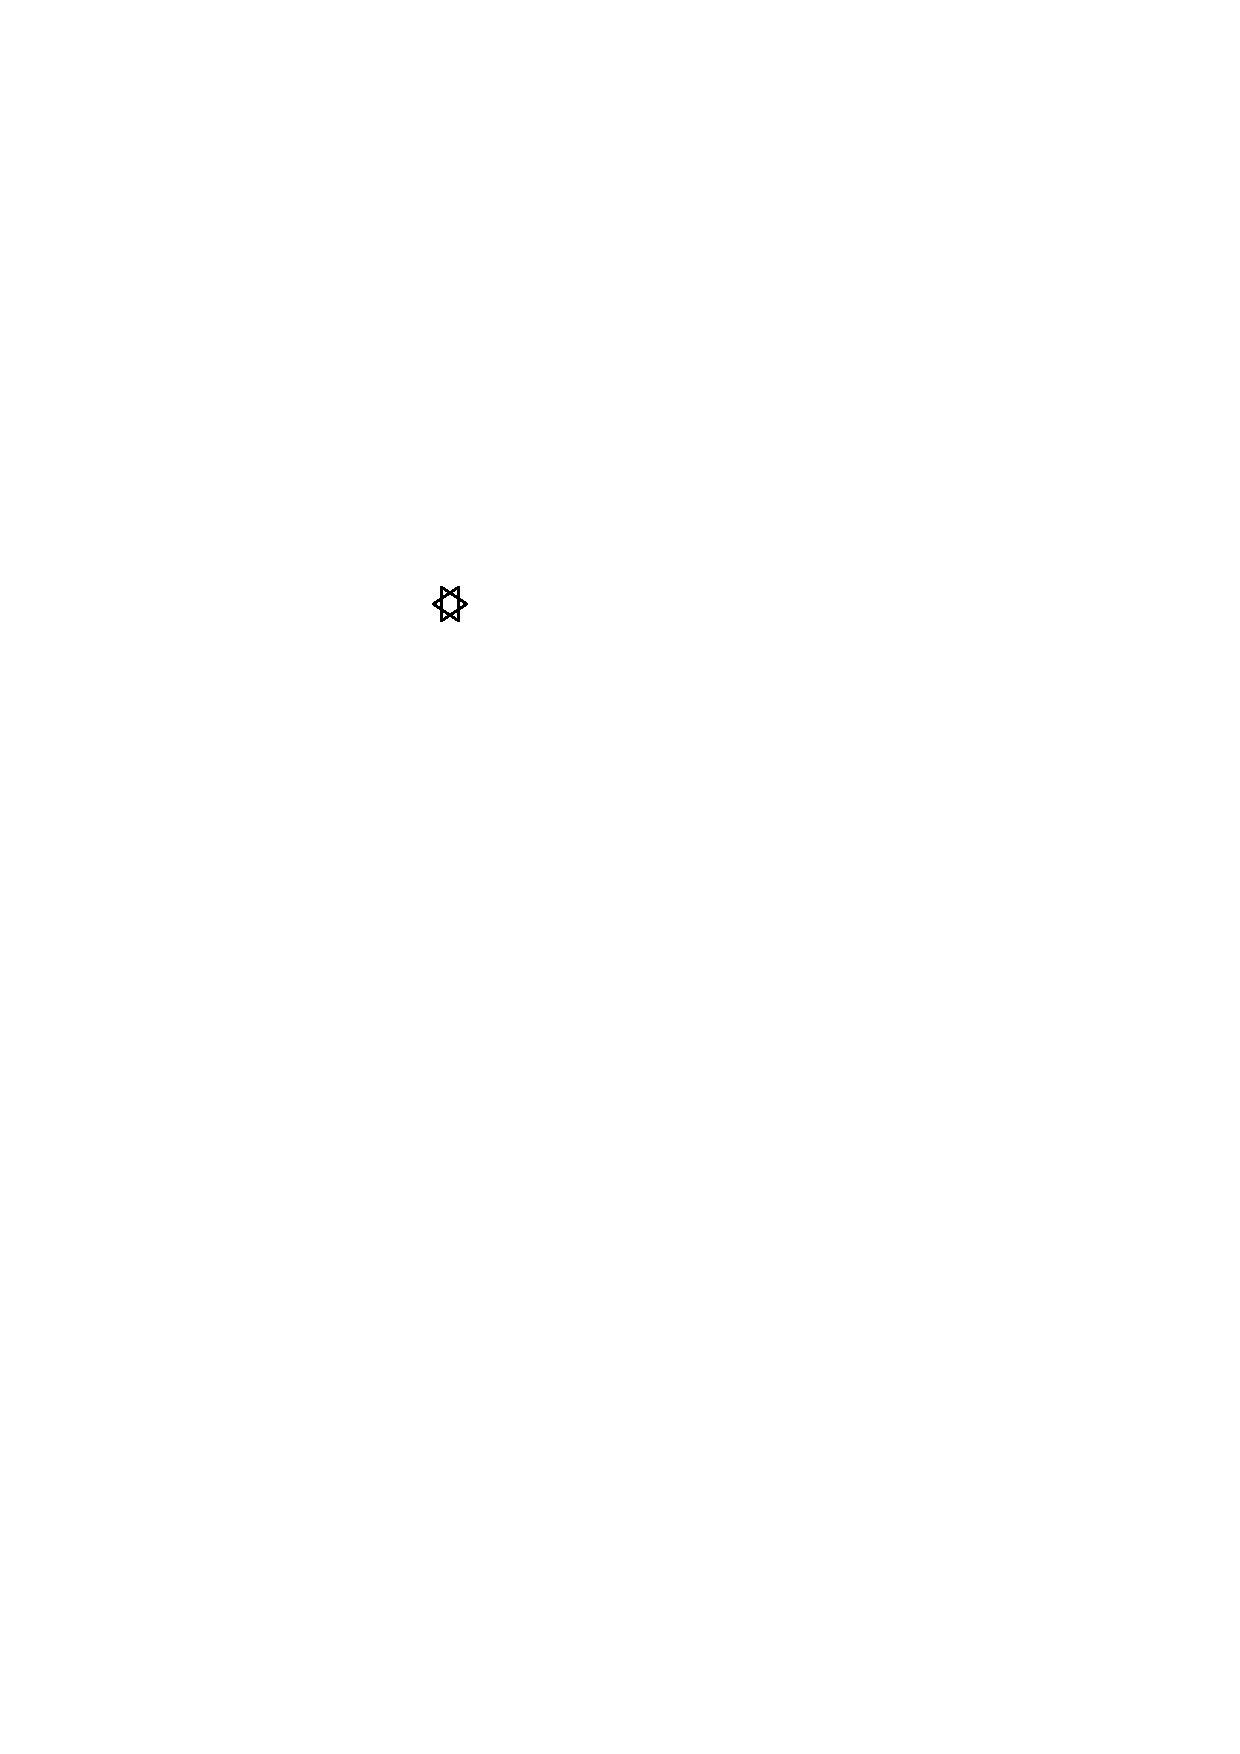
\includegraphics[height=2.0ex]{figs/triangles-disjoint-3}}}


\newcommand{\mi}[1]{\multiinclude[<+>][start=1,format=pdf]{#1}}

\DeclareMathOperator{\ex}{ex}

 
\usepackage{amsthm}

\newcommand{\centeripe}[1]{\begin{center}\Ipe{#1}\end{center}}
\newcommand{\comment}[1]{}

\newcommand{\centerpsfig}[1]{\centerline{\psfig{#1}}}

\newcommand{\seclabel}[1]{\label{sec:#1}}
\newcommand{\Secref}[1]{Section~\ref{sec:#1}}
\newcommand{\secref}[1]{\mbox{Section~\ref{sec:#1}}}

\newcommand{\alglabel}[1]{\label{alg:#1}}
\newcommand{\Algref}[1]{Algorithm~\ref{alg:#1}}
\newcommand{\algref}[1]{\mbox{Algorithm~\ref{alg:#1}}}

\newcommand{\applabel}[1]{\label{app:#1}}
\newcommand{\Appref}[1]{Appendix~\ref{app:#1}}
\newcommand{\appref}[1]{\mbox{Appendix~\ref{app:#1}}}

\newcommand{\tablabel}[1]{\label{tab:#1}}
\newcommand{\Tabref}[1]{Table~\ref{tab:#1}}
\newcommand{\tabref}[1]{Table~\ref{tab:#1}}

\newcommand{\figlabel}[1]{\label{fig:#1}}
\newcommand{\Figref}[1]{Figure~\ref{fig:#1}}
\newcommand{\figref}[1]{\mbox{Figure~\ref{fig:#1}}}

\newcommand{\eqlabel}[1]{\label{eq:#1}}
%\newcommand{\eqref}[1]{(\ref{eq:#1})}
\newcommand{\Eqref}[1]{Equation~(\ref{eq:#1})}

\newtheorem{thm}{Theorem}{\bfseries}{\itshape}
\newcommand{\thmlabel}[1]{\label{thm:#1}}
\newcommand{\thmref}[1]{Theorem~\ref{thm:#1}}

\newtheorem{lem}{Lemma}{\bfseries}{\itshape}
\newcommand{\lemlabel}[1]{\label{lem:#1}}
\newcommand{\lemref}[1]{Lemma~\ref{lem:#1}}

\newtheorem{cor}{Corollary}{\bfseries}{\itshape}
\newcommand{\corlabel}[1]{\label{cor:#1}}
\newcommand{\corref}[1]{Corollary~\ref{cor:#1}}

\newtheorem{obs}{Observation}{\bfseries}{\itshape}
\newcommand{\obslabel}[1]{\label{obs:#1}}
\newcommand{\obsref}[1]{Observation~\ref{obs:#1}}

\newtheorem{cond}{Condition}{\bfseries}{\itshape}

\newtheorem{clm}{Claim}{\bfseries}{\itshape}
\newcommand{\clmlabel}[1]{\label{clm:#1}}
\newcommand{\clmref}[1]{Claim~\ref{clm:#1}}


\newtheorem{dfn}{Definition}{\bfseries}{\rm}

\newtheorem{assumption}{Assumption}{\bfseries}{\rm}
\newenvironment{ass}{\begin{assumption}\rm}{\end{assumption}}
\newcommand{\asslabel}[1]{\label{ass:#1}}
\newcommand{\assref}[1]{Assumption~\ref{ass:#1}}

\newcommand{\proclabel}[1]{\label{alg:#1}}
\newcommand{\procref}[1]{Procedure~\ref{alg:#1}}

\newtheorem{rem}{Remark}
\newtheorem{op}{Open Problem}

\newcommand{\etal}{\emph{et al}}

%\newcommand{\keywords}[1]{\noindent\textbf{Keywords:} #1}
\newcommand{\voronoi}{Vorono\u\i}
\newcommand{\ceil}[1]{\left\lceil #1 \right\rceil}
\newcommand{\floor}[1]{\left\lfloor #1 \right\rfloor}
\newcommand{\R}{\mathbb{R}}
\newcommand{\N}{\mathbb{N}}
\newcommand{\Z}{\mathbb{Z}}
\newcommand{\Sp}{\mathbb{S}}
\newcommand{\E}{\mathrm{E}}

\usepackage{marvosym}

\newcommand{\notice}[1]
{
   {\Lightning}
   \marginpar{
      \begin{flushleft}\raggedright
        \hspace{-1.5mm}\Lightning{\small #1}
      \end{flushleft}
   }
}



\title{Turán-Type Theorems for Triangles \newline in Convex Point Sets}
\author{Pat Morin}
\date{Shonan Village Meeting \\ May 30, 2016}

\begin{document}

\begin{frame}
  \titlepage
\end{frame}


\begin{frame}
   \frametitle{$\ex(n,\{\taco,\nested\})$}
%   \framesubtitle{
%      %\newlength{\ka}
%      \setlength{\ka}{.3\textwidth}
%      \addtolength{\ka}{-1cm}
%      \begin{tabular}{c@{\hspace{1cm}}c}
%        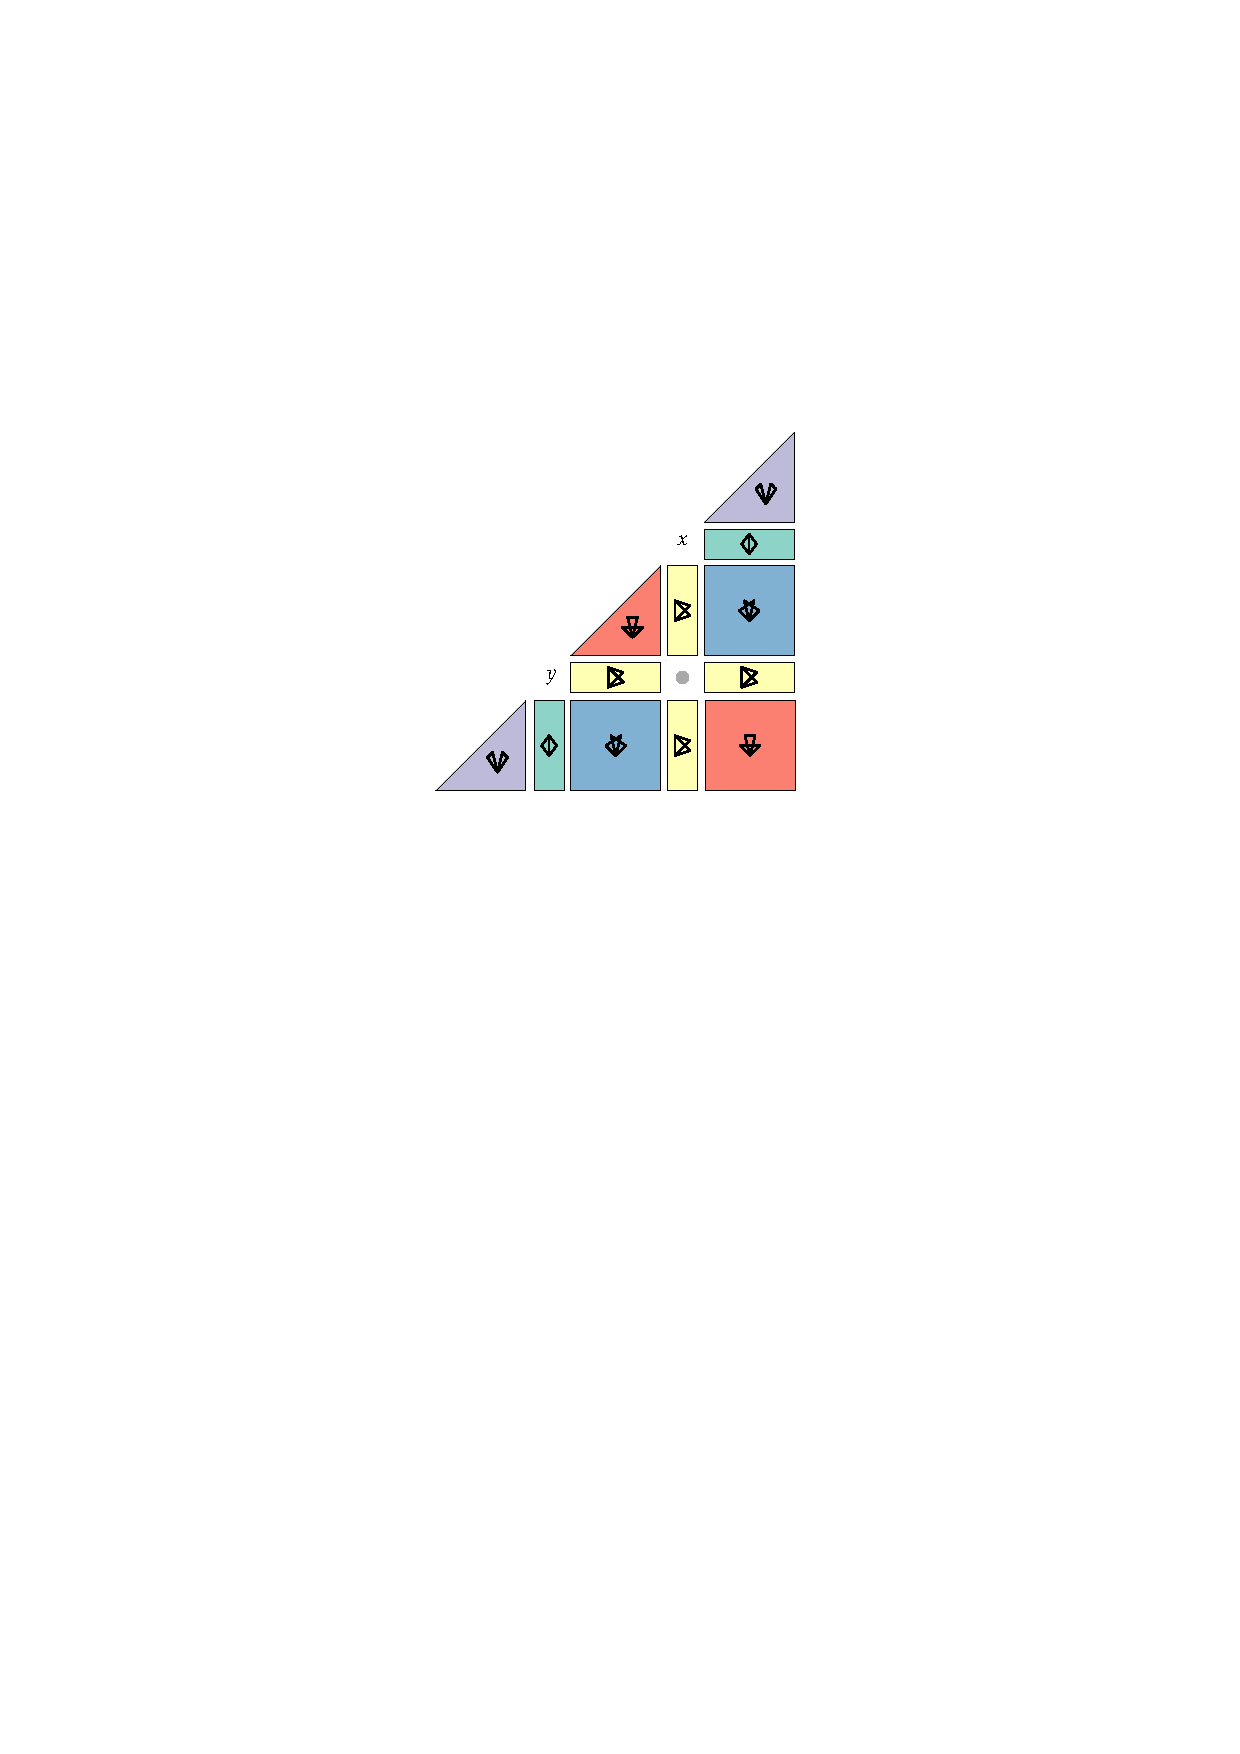
\includegraphics[width=.48\ka]{figs/crapper-2} & 
%        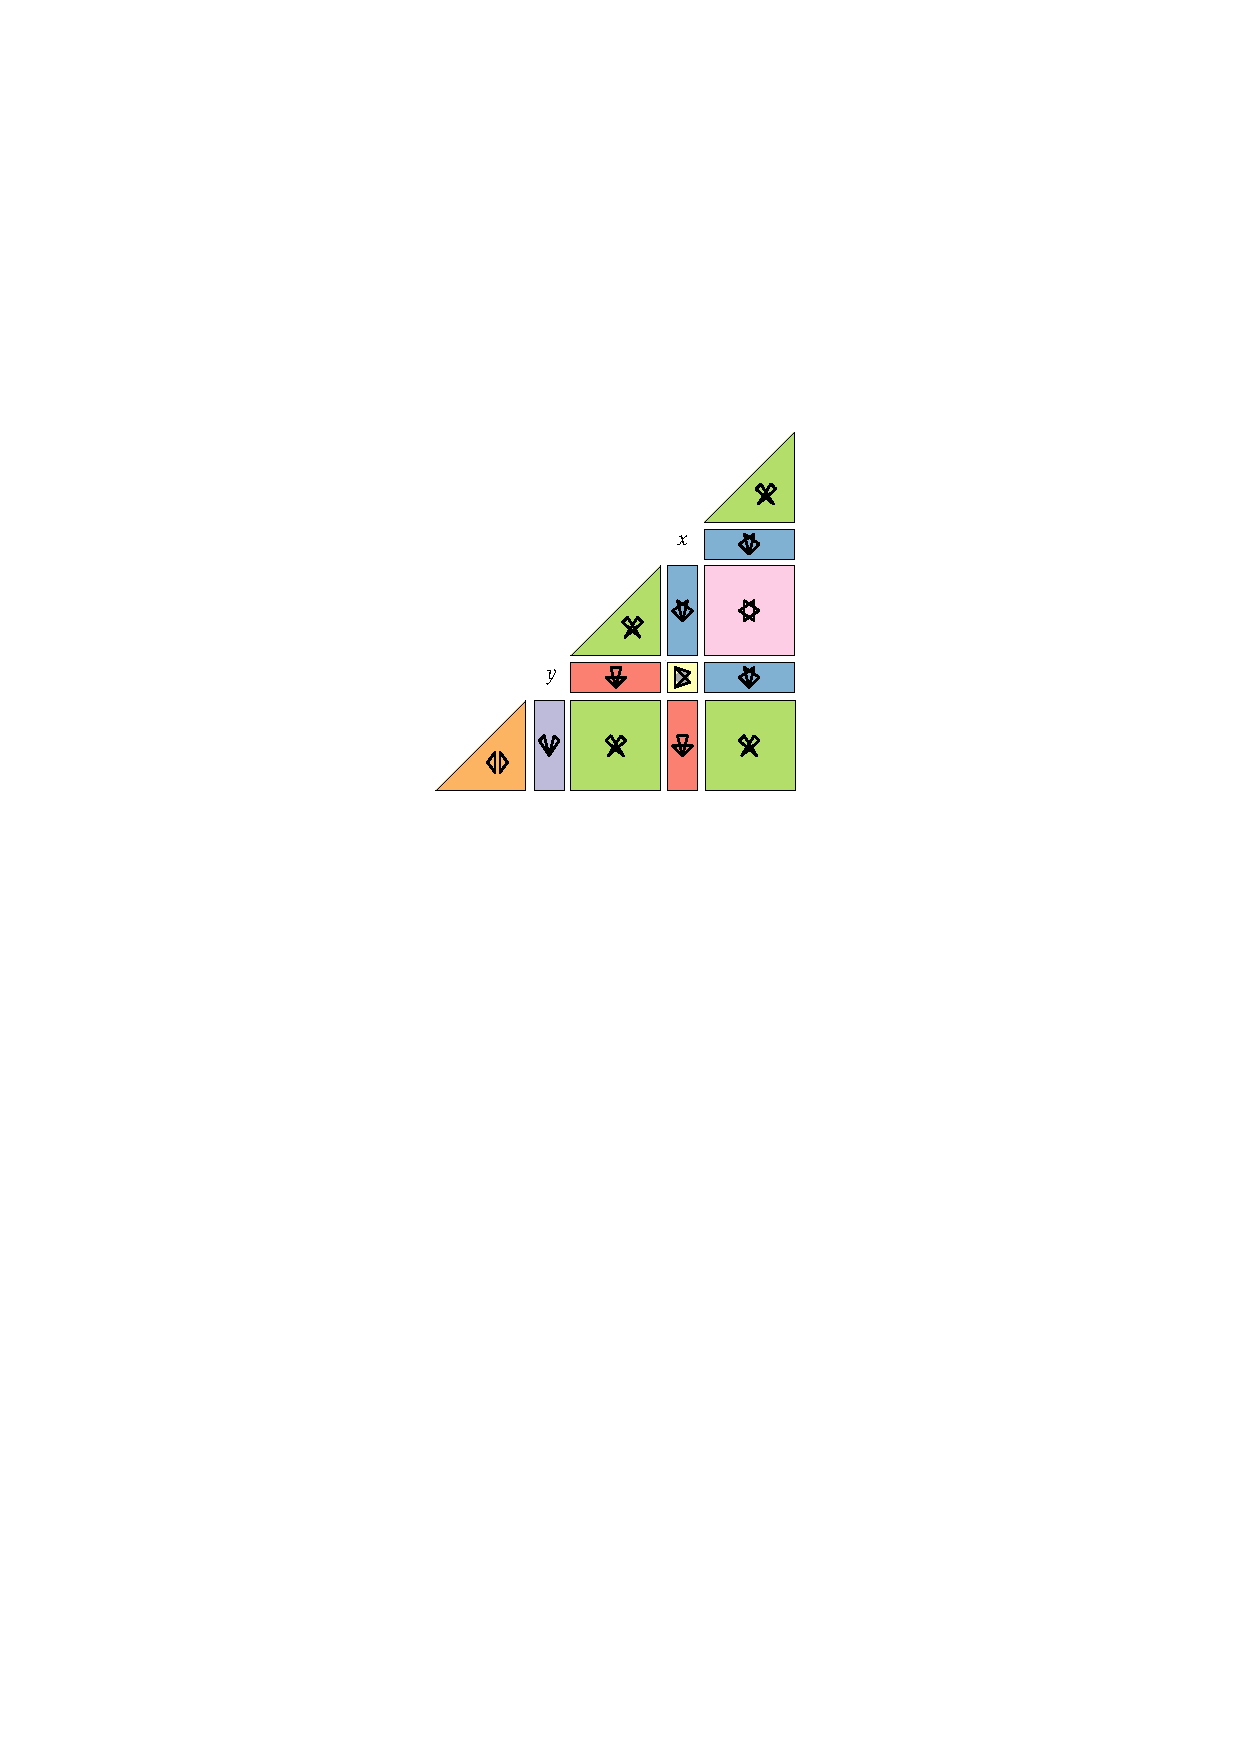
\includegraphics[width=.48\ka]{figs/crapper-1} 
%      \end{tabular}
%   }
   \begin{itemize}
      %\item<1-> We know $\ex'(n,X)$ for every $X$ of size 2 except
      %  $X=\{\taco,\nested\}$
      %\item<1-> Posed in Bra\ss\ 2004
      \item<1-> A puzzle played in $n$ rounds on the $n\times n$ grid
      \item<2-> Within each round, points must form an increasing sequence
      \item<3-> Each point kills a {\raisebox{-.1ex}{\includegraphics[angle=180,origin=c,height=2.0ex]{slidefigs/shape}}}
 shape that can't be played in subsequent rounds
      \item<4-> The goal is to play as many points as possible
%      \item<4-> $\Omega(n^{3/2})$ lower bound is easy (and looks tight):\\
%      \begin{center}
%        \only<1-4>{\includegraphics{slidefigs/n32-1}}%
%        \only<5>{\includegraphics{slidefigs/n32-2}}%
%        \only<6>{\includegraphics{slidefigs/n32-3}}%
%        \only<7>{\includegraphics{slidefigs/n32-4}}%
%        \only<8>{\includegraphics{slidefigs/n32-5}}%
%        \only<9>{\includegraphics{slidefigs/n32-6}}%
%        \only<10->{\includegraphics{slidefigs/n32-7}}%
%      \end{center}
      %\item<11-> We have no upper bound better than $O(n^2)$
   \end{itemize}
\end{frame}

\begin{frame}
   \frametitle{$\ex(n,\{\taco,\nested\})\in\omega(n^{3/2})$}
   \begin{itemize}
       %\item Ignoring constant factors, we can assume a $n\times n$ board
       %\item Rotating, each point kills an L shape
       \centerline{\mi{slidefigs/sqrtn}}%
       \item $\only<2->{3}
              \only<4->{+3}
              \only<6->{+3}
              \only<8->{+3}
              \only<10->{+3}
              \only<12->{+3}
              \only<14->{+3}
              \only<16->{+3}
              \only<18->{+3}
              \only<19->{=27=9^{3/2}}
             $
   \end{itemize}
\end{frame}


\begin{frame}
   \frametitle{$\ex(n,\{\taco,\nested\})\in\omega(n^{3/2})$}
   \begin{itemize}
       \item Another strategy:
       \centerline{\mi{slidefigs/sqrtn-david}}%
       \item $\only<2->{3}
              \only<3->{+3}
              \only<4->{+3}
              \only<5->{+3}
              \only<6->{+3}
              \only<7->{+3}
              \only<8->{+3}
              \only<9->{+3}
              \only<10->{+3}
              \only<11->{=27=9^{3/2}}
             $
   \end{itemize}
\end{frame}


\begin{frame}
   \frametitle{$\ex(n,\{\taco,\nested\})\in\omega(n^{3/2})$}
   \begin{itemize}
       \item A third try:
       \centerline{\mi{slidefigs/nine-twentyeight}}%
       \item $\only<2->{3}
              \only<3->{+3}
              \only<4->{+3}
              \only<5->{+3}
              \only<6->{+{\color{red}4}}
              \only<7->{+3}
              \only<8->{+3}
              \only<9->{+3}
              \only<10->{+3}
              \only<11->{=28=9^{1.516551628}}
             $
   \end{itemize}
\end{frame}

\begin{frame}
   \frametitle{$\ex(n,\{\taco,\nested\})\in\omega(n^{3/2})$}
   \begin{itemize}
       \item For general $n$, use recursion on subproblems of size $(n/9)\times(n/9)$
       \centerline{\includegraphics[scale=0.8]{slidefigs/recursion}}%
       \item[] \[ T(n) = \begin{cases}
                 28 & \text{if $n=9$} \\
                 28 T(n/9) & \text{if $n=9^k$} \end{cases} \]
       \item $ T(n) = \Theta(n^{\log_9 28}) = \Theta(n^{1.516551628})$
   \end{itemize}
\end{frame}


\begin{frame}
   \frametitle{$\ex(n,\{\taco,\nested\})$}

   \begin{itemize}[<+->]
      \item Can we do better than $\Theta(n^{1.516551628})$?
      \item $70\times70$ game has an $652$ point solution
      \item Recursion gives $\Omega(n^{1.5252564009\ldots})$ solution for $n\times n$
      \item That's the best lower-bound we have so far\ldots
   \end{itemize} 
\end{frame}

\begin{frame}
   \frametitle{$\ex(n,\{\taco,\nested\})$---Upper Bounds}

   \begin{itemize}[<+->]
      \item $O(n^2)$ upper bound is trivial.
      \item Treat $x$ and $y$ coordinates as vertices of a bipartite graph, $G$
      \item Each round, $i$, becomes a matching, $M_i$
      \item No edge from $M_j$, $j\neq i$, joins two vertices used in $M_i$. \\[1ex]
        \centerline{\includegraphics{slidefigs/induced}}
      \item Puzzle solution gives a solution to the \emph{Rusza-Szemerédi Induced Matching Problem}
      \begin{itemize}
         \item Puzzle score $=|E(G)|$ 
      \end{itemize}
      \item IM Problem has an $O(n^{2/e^{\log^* n}})$ upper bound
      \item Maximum puzzle score is $O(n^2/e^{\log^* n})$
   \end{itemize} 
\end{frame}



\begin{frame}
  \frametitle{Maximum Triangles Problem}
  \framesubtitle{Erd\H{o}s and Purdy (1971)}

  \begin{itemize}
      \item What is the largest number of maximum area triangles determined by a set of $n$ points?\\[1ex]
      \centerline{\mi{slidefigs/erdos-regular}}%
      \item<2->Answer: At least $n$
  \end{itemize}
\end{frame}

\begin{frame}
  \frametitle{Maximum Triangles Problem}
  \framesubtitle{Bra\ss, Rote, Swanepoel (2001)}

  \only<+->{
  \textbf{Theorem:} Any set of $n$ points determines at most $n$ maximum-area triangles}
  \begin{itemize}[<+->]
      \item WLOG we can assume points are in convex position
      \item How can a pair of maximum area triangles interleave?
      \begin{itemize}
         \item Boyce, Dobkin, Drysdale, Guibas (1985)
         \item Like this: \taco, \david, \crossing, \mariposa
         \item Not like this: \ears, \swords, \nested, \bat
      \end{itemize}
      \item What is the maximum number of triangles we can draw on a convex
         $n$-gon before we
         get a pair like  \ears, \swords, \nested, or \bat?
      \item No geometry!
  \end{itemize}
\end{frame}

\begin{frame}
  \frametitle{Maximum Triangles Problem}
  \framesubtitle{Bra\ss, Rote, Swanepoel (2001)}

  Let $\ex(n,X)$ denote the maximum number of triangles we can draw on a convex $n$-gon before we get a configuration from $X$.\\[2ex]

  \uncover<2->
  {\textbf{Theorem (BRS2001):} $\ex(n,\{\ears,\swords,\nested,\bat\})\le n$.}

%  \begin{itemize}
%     \item<3-> Number polygon vertices $0,\ldots,n-1$
%     \item<4-> Represent each triangle as a triple: $(a,b,c)$, with $0\le a<b<c<n$.
%     \item<5-> Partially-order triangles according to 
%         \[ (x_1,y_1,z_1)\preceq (x_2,y_2,z_2) \Leftrightarrow x_1\le x_2, y_1\le y_2, z_1\le z_2 \] 
%     \item<6-> Key insight: Any pair of maximum-area triangles (\taco, \david, \crossing, \mariposa) is comparable! 
%     \item<7-> $\Delta_1<\Delta_2<\cdots<\Delta_k \Rightarrow k < 3n$
%     \item<8-> Count a bit more carefully to get $k\le n$ \hfill{QED}
%  \end{itemize}
\end{frame} 

\begin{frame}
  \frametitle{Turán-Type Theorems for Triangles in Convex Point Sets}
  \framesubtitle{256 Problems}

   \begin{itemize}[<+->]
      \item $\ex(n,X)$ is the maximum number of triangles we can draw on 
         a convex $n$-gon before we get a configuration from $X$
 
      \item 256 problems: Determine $\ex(n,X)$ for every $X\subseteq\{\taco,\david,\crossing,\mariposa,\ears,\swords,\nested,\bat\}$
   \end{itemize}
\end{frame}

\begin{frame}
   \frametitle{Bra\ss\ 2004}
      Bra\ss\ (2004): 
        \[ \begin{array}{rrr}
           \ex(n,\{\ears\})=\Theta(n^3) & \ex(n,\{\swords\})=\Theta(n^2) & \ex(n,\{\david\})=\Theta(n^2) \\
           \ex(n,\{\bat\})=\Theta(n^3) & \ex(n,\{\nested\})=\Theta(n^2) & \ex(n,\{\crossing\})=\Theta(n^2) \\
           \ex(n,\{\mariposa\})=\Theta(n^3) & \ex(n,\{\taco\})=\Theta(n^2) 
           \end{array}
        \]
        \[\begin{array}{r}
           \ex(n,\{\bat,\nested\})=\Theta(n^2) \\ \ex(n,\{\crossing,\nested\})=\Theta(n^2) \\ \ex(n,\{\bat,\crossing\})=\Theta(n^2) \\
        \end{array}\]
\end{frame}

\begin{frame}
  \frametitle{Proof that $\ex(n,\{\crossing\})=O(n^2)$}
  \framesubtitle{Bra\ss\ (2004)}

  \centerline{\mi{slidefigs/crossing}}

  \uncover<4->{\hfill{QED}}
\end{frame} 


\begin{frame}
  \frametitle{Proof that $\ex(n,\{\swords\})=O(n^2)$}
  \framesubtitle{Bra\ss (2004)}

  \centerline{\mi{slidefigs/swords}}
  \begin{itemize}[<4->]
      \item[]\ \hfill{QED}
  \end{itemize}

\end{frame} 


\begin{frame}
  \frametitle{Proof that $\mariposa$ doesn't matter}

   \textbf{Theorem:} Any set of triangles of size $N$ contains a subset
    of size at least $N/8$ that has no \mariposa\ pair
  \begin{itemize}
   \item<2-> Randomly direct each pair $(u,v)$ of vertices ($\overrightarrow{uv}$ or $\overleftarrow{uv}$)
   \item<3-> Discard all triangles that use $uv$ and are on the right of $uv$
  \end{itemize}
   \centerline{
       \only<1>{\includegraphics{slidefigs/chucker-1}}%
       \only<2>{\includegraphics{slidefigs/chucker-2}}%
       \only<3->{\includegraphics{slidefigs/chucker-3}}%
    }
  \begin{itemize}[<4->]
   \item Resulting set has expected size $N/8$ and no $\mariposa$ pairs
     \hfill{QED}
  \end{itemize} 
\end{frame} 


\begin{frame}
  \frametitle{The Top-Bottom View}

   Define $\ex'(n,X)$ just like $\ex(n,X)$ but only count triangles
   with one vertex in the bottom half and two in the top half.

   \centerline{\includegraphics{slidefigs/top-bottom}}

\uncover<2->{
\textbf{Lemma:}
  If $\ex'(n,X)\in O(n^c)$, then
  \[
     \ex(n,X)\in 
        \begin{cases} 
            O(n^c)     & \text{if $c>1$} \\
            O(n\log n) & \text{if $c=1$}
        \end{cases}
  \]
}
\uncover<3>{
  \emph{Proof:} $\ex(n)\le 2\ex'(n) + 2\ex(n/2)$
}
\end{frame} 


\begin{frame}
    \frametitle{The Dot-Puzzle View}
    \framesubtitle{A One-Player Game}

    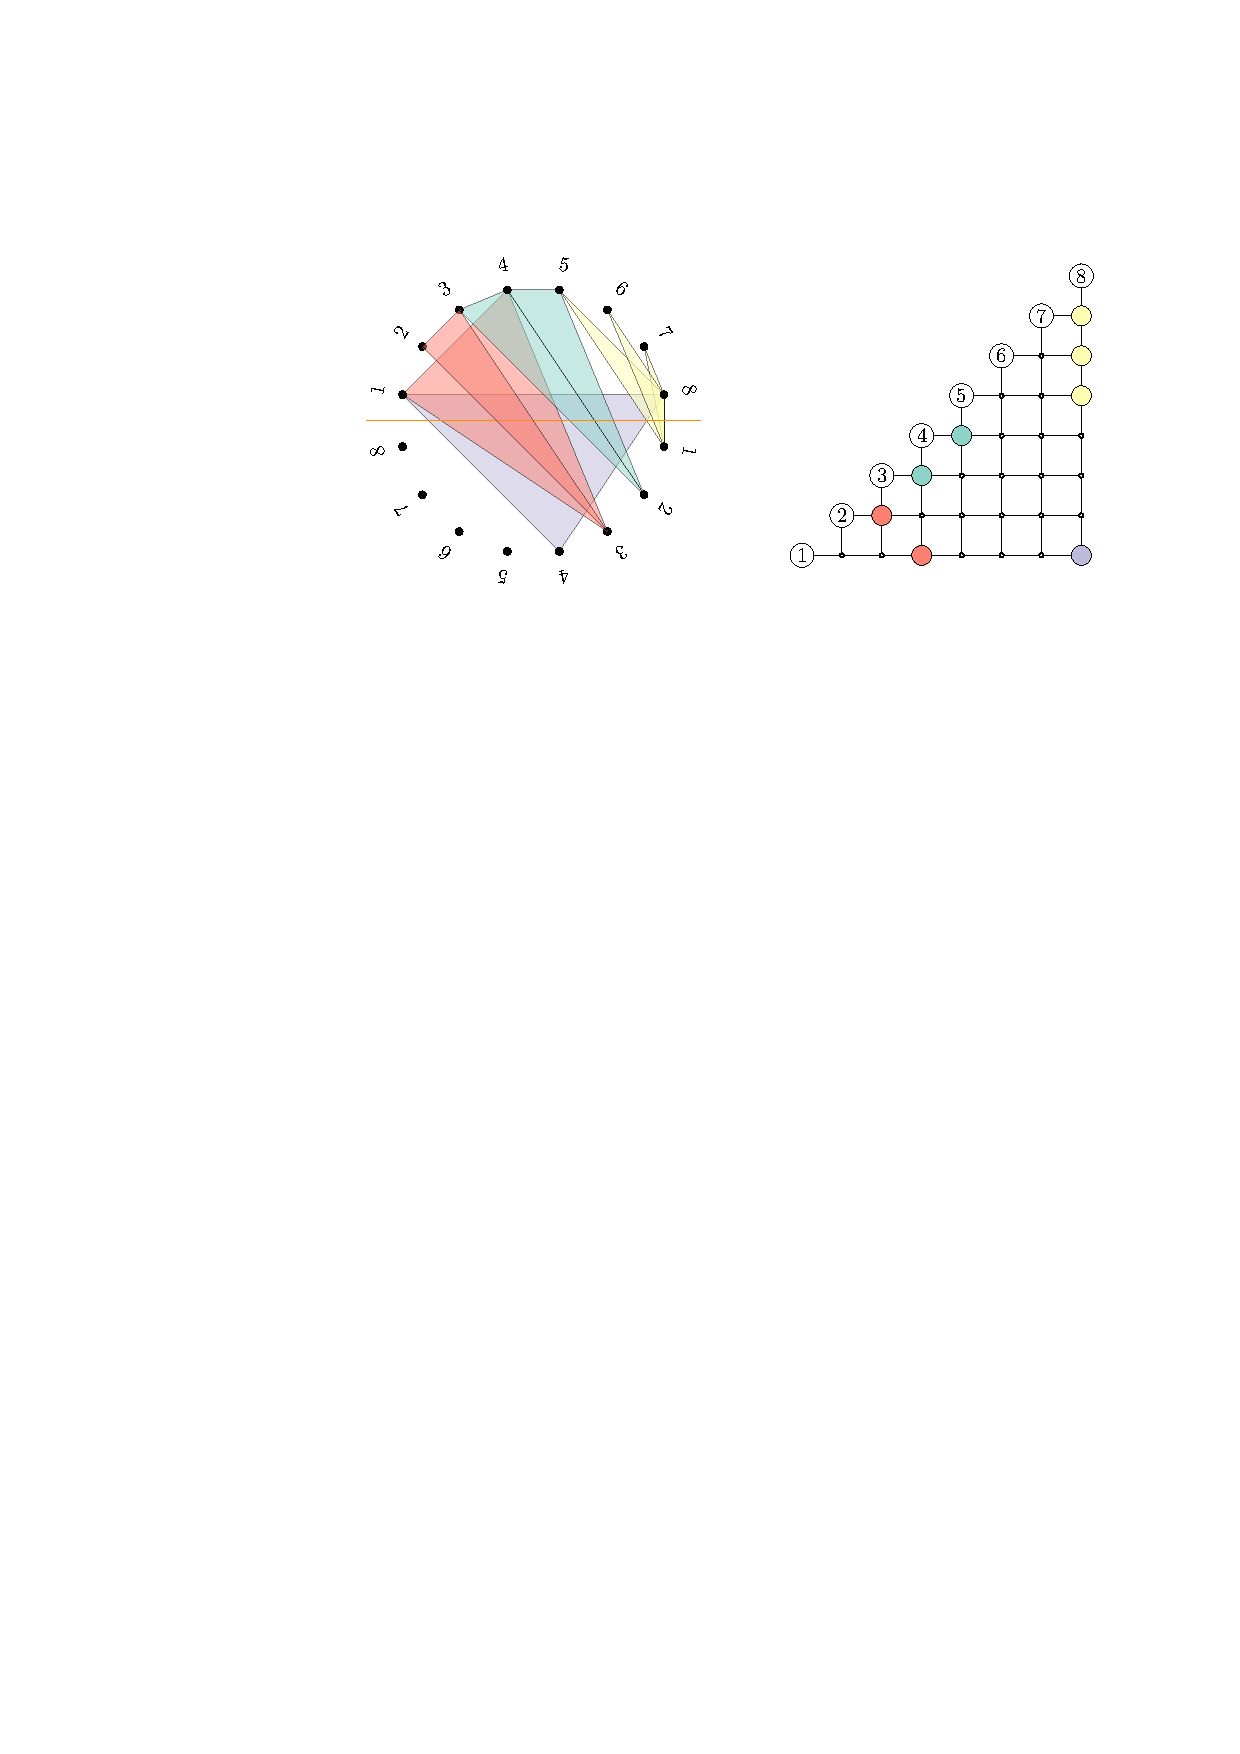
\includegraphics[width=.95\textwidth]{figs/point-view}
    \uncover<2->{\begin{center}A puzzle played in $n$ rounds\end{center}}
\end{frame}

\begin{frame}
    \frametitle{The Dot-Puzzle View}
    \framesubtitle{The Rules}

   \begin{center}
      \newlength{\ka}
      \setlength{\ka}{\textwidth}
      \addtolength{\ka}{-1cm}
      \begin{tabular}{c@{\hspace{1cm}}c}
        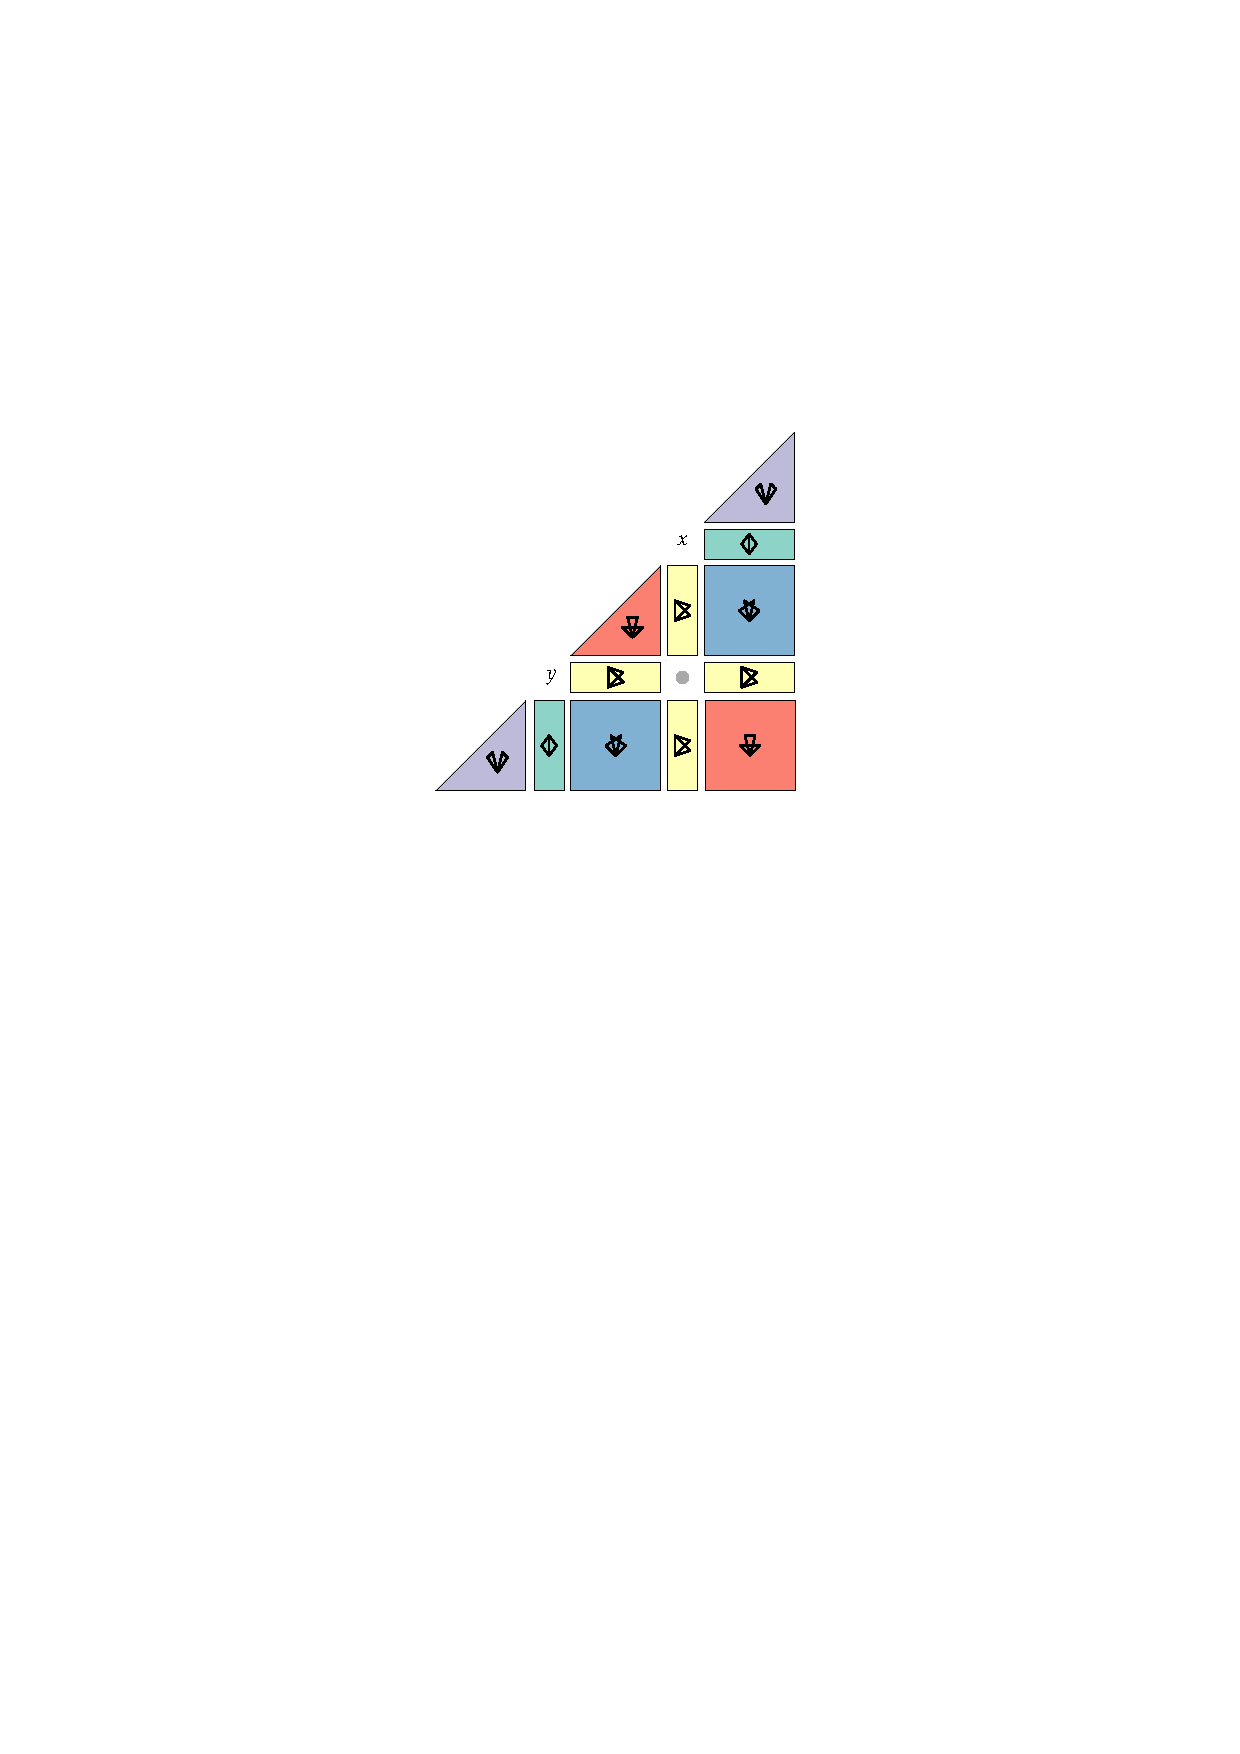
\includegraphics[width=.48\ka]{figs/crapper-2} & 
        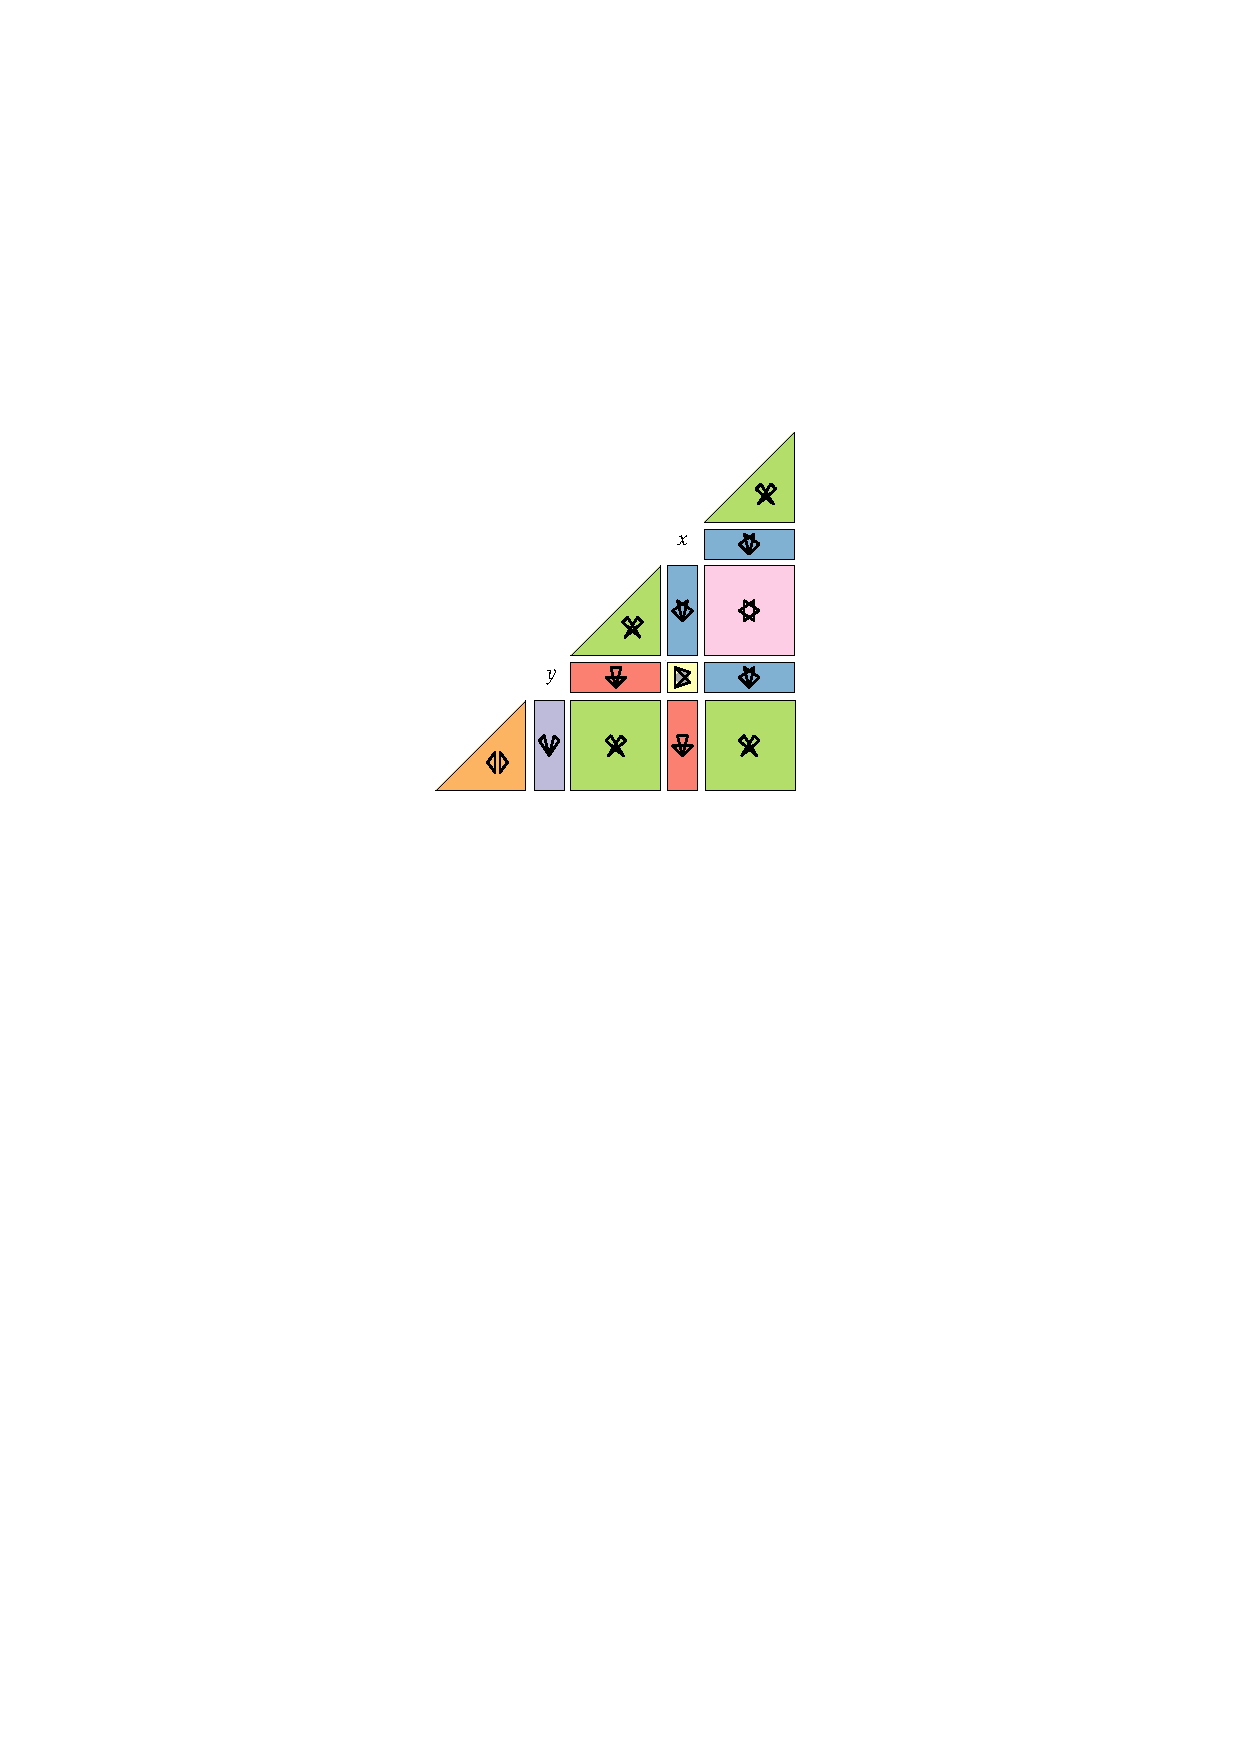
\includegraphics[width=.48\ka]{figs/crapper-1} \\
        within round & subsequent rounds
      \end{tabular}
   \end{center}
\end{frame}

\begin{frame}
   \frametitle{\swords\ is a killer}
   \framesubtitle{
      %\newlength{\ka}
      \setlength{\ka}{.3\textwidth}
      \addtolength{\ka}{-1cm}
      \begin{tabular}{c@{\hspace{1cm}}c}
        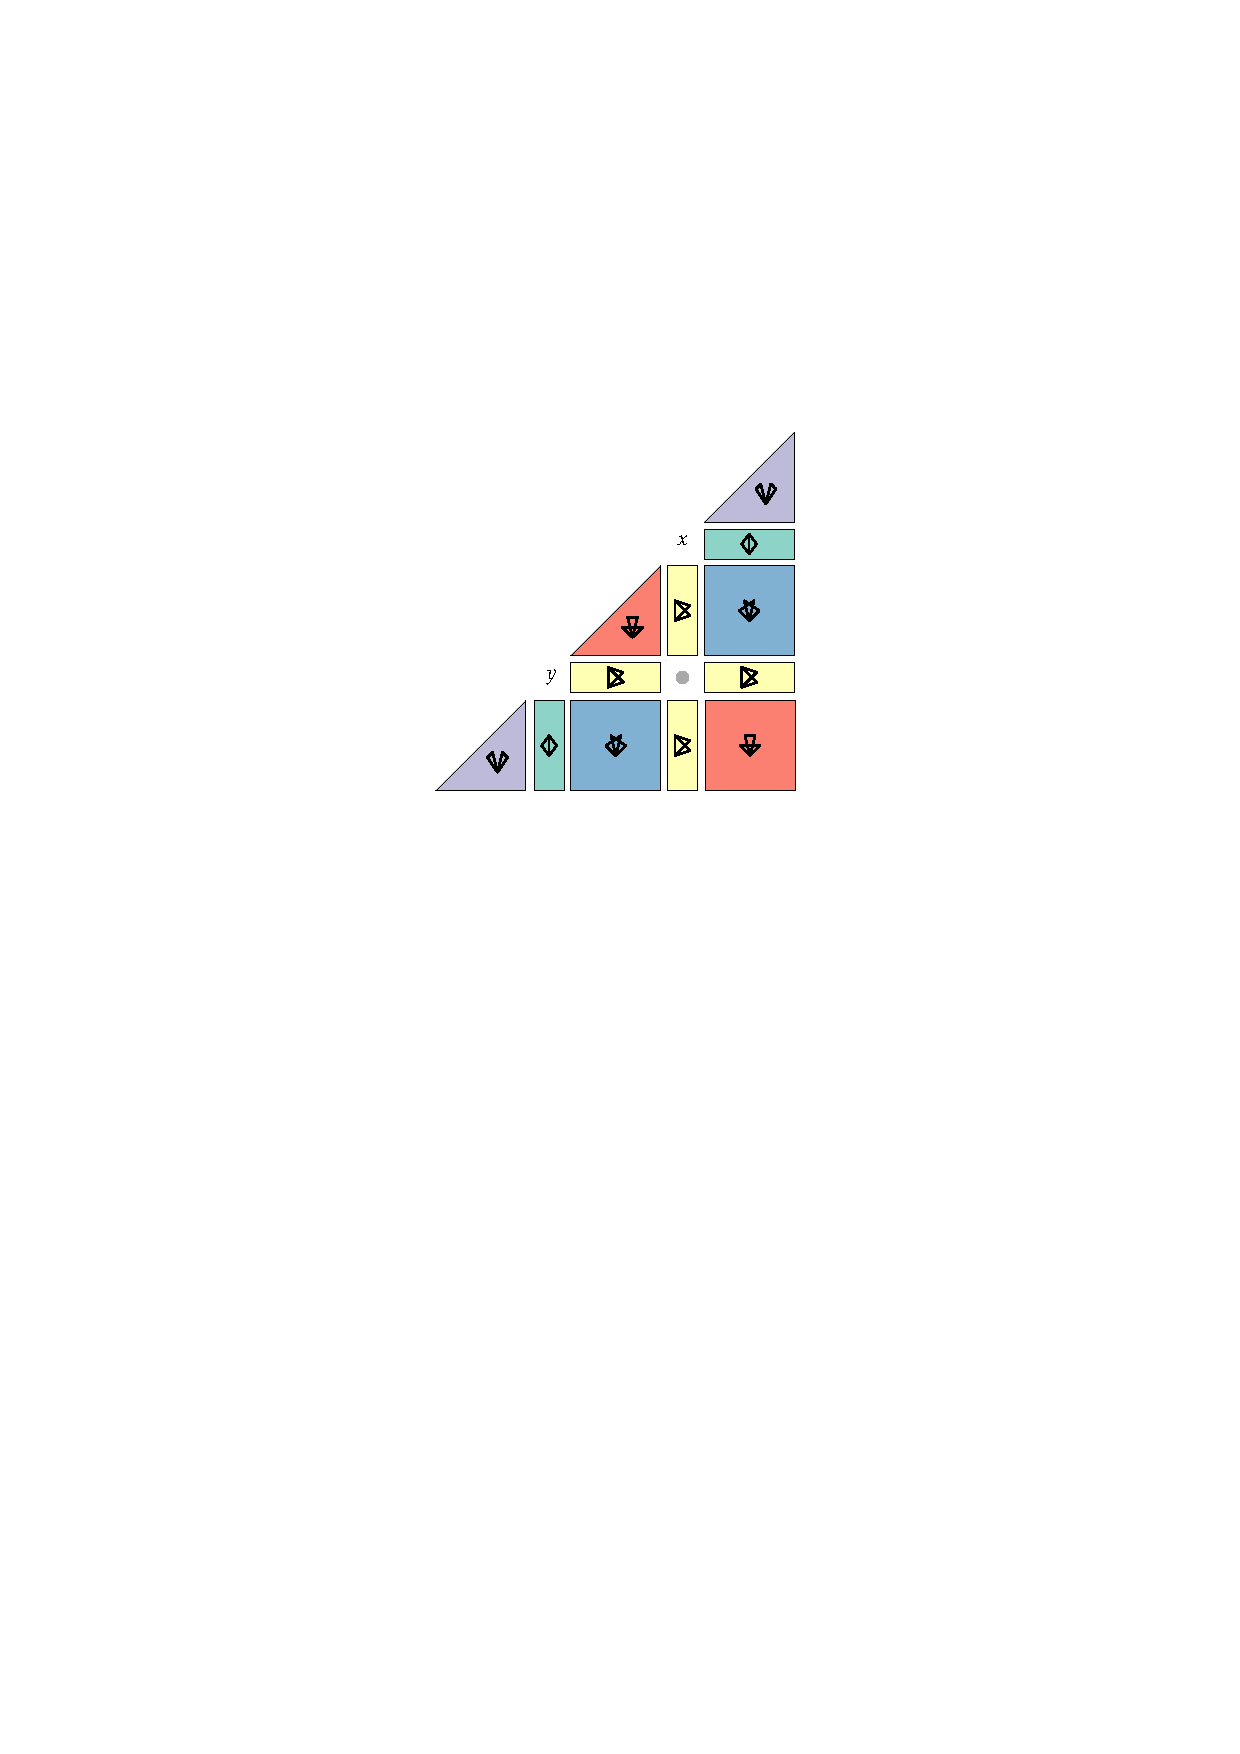
\includegraphics[width=.48\ka]{figs/crapper-2} & 
        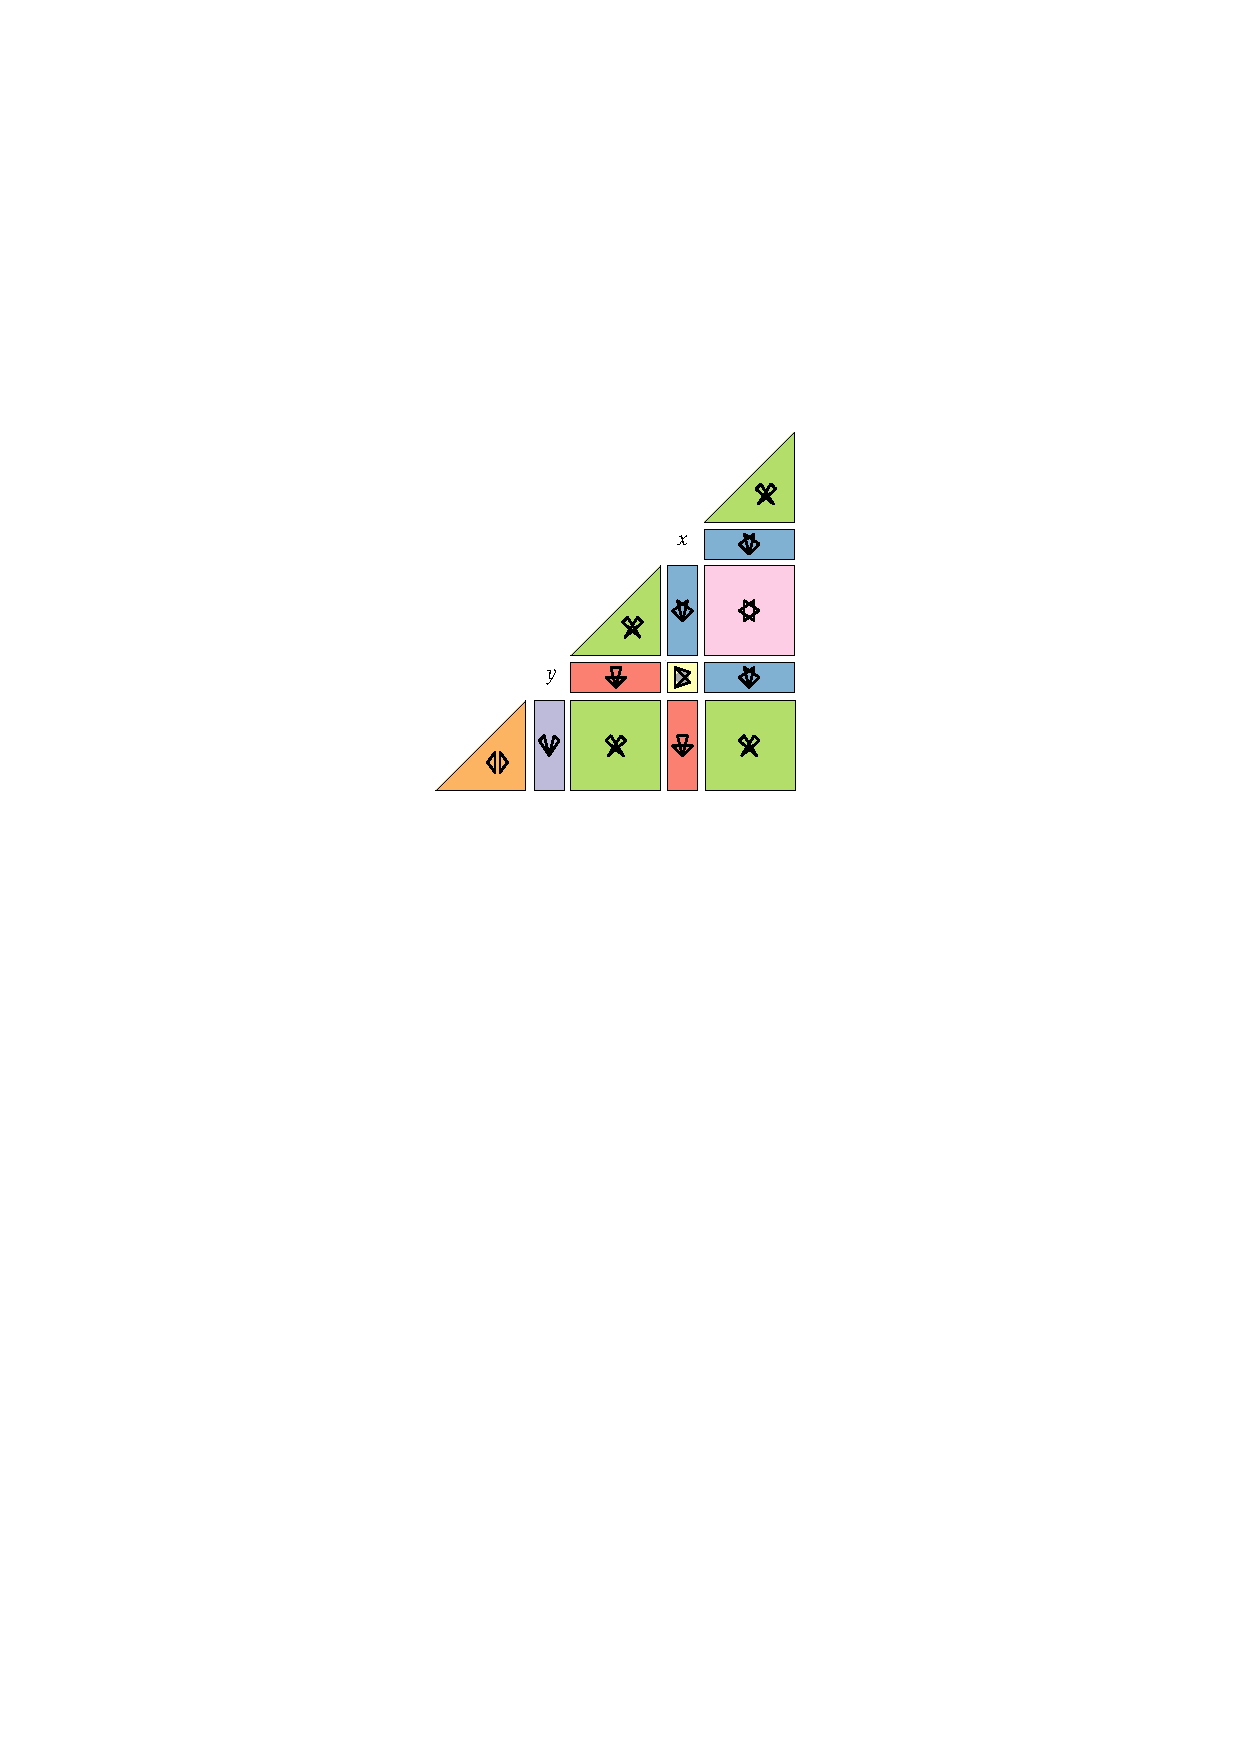
\includegraphics[width=.48\ka]{figs/crapper-1} 
      \end{tabular}
   }
   \centerline{\includegraphics{slidefigs/swords-region-1}}
   \invisible<1->{\hfill{QED}}
\end{frame}

\begin{frame}
   \frametitle{$\ex'(n,\{\swords,\taco\})=O(n)$}
   \framesubtitle{
      %\newlength{\ka}
      \setlength{\ka}{.3\textwidth}
      \addtolength{\ka}{-1cm}
      \begin{tabular}{c@{\hspace{1cm}}c}
        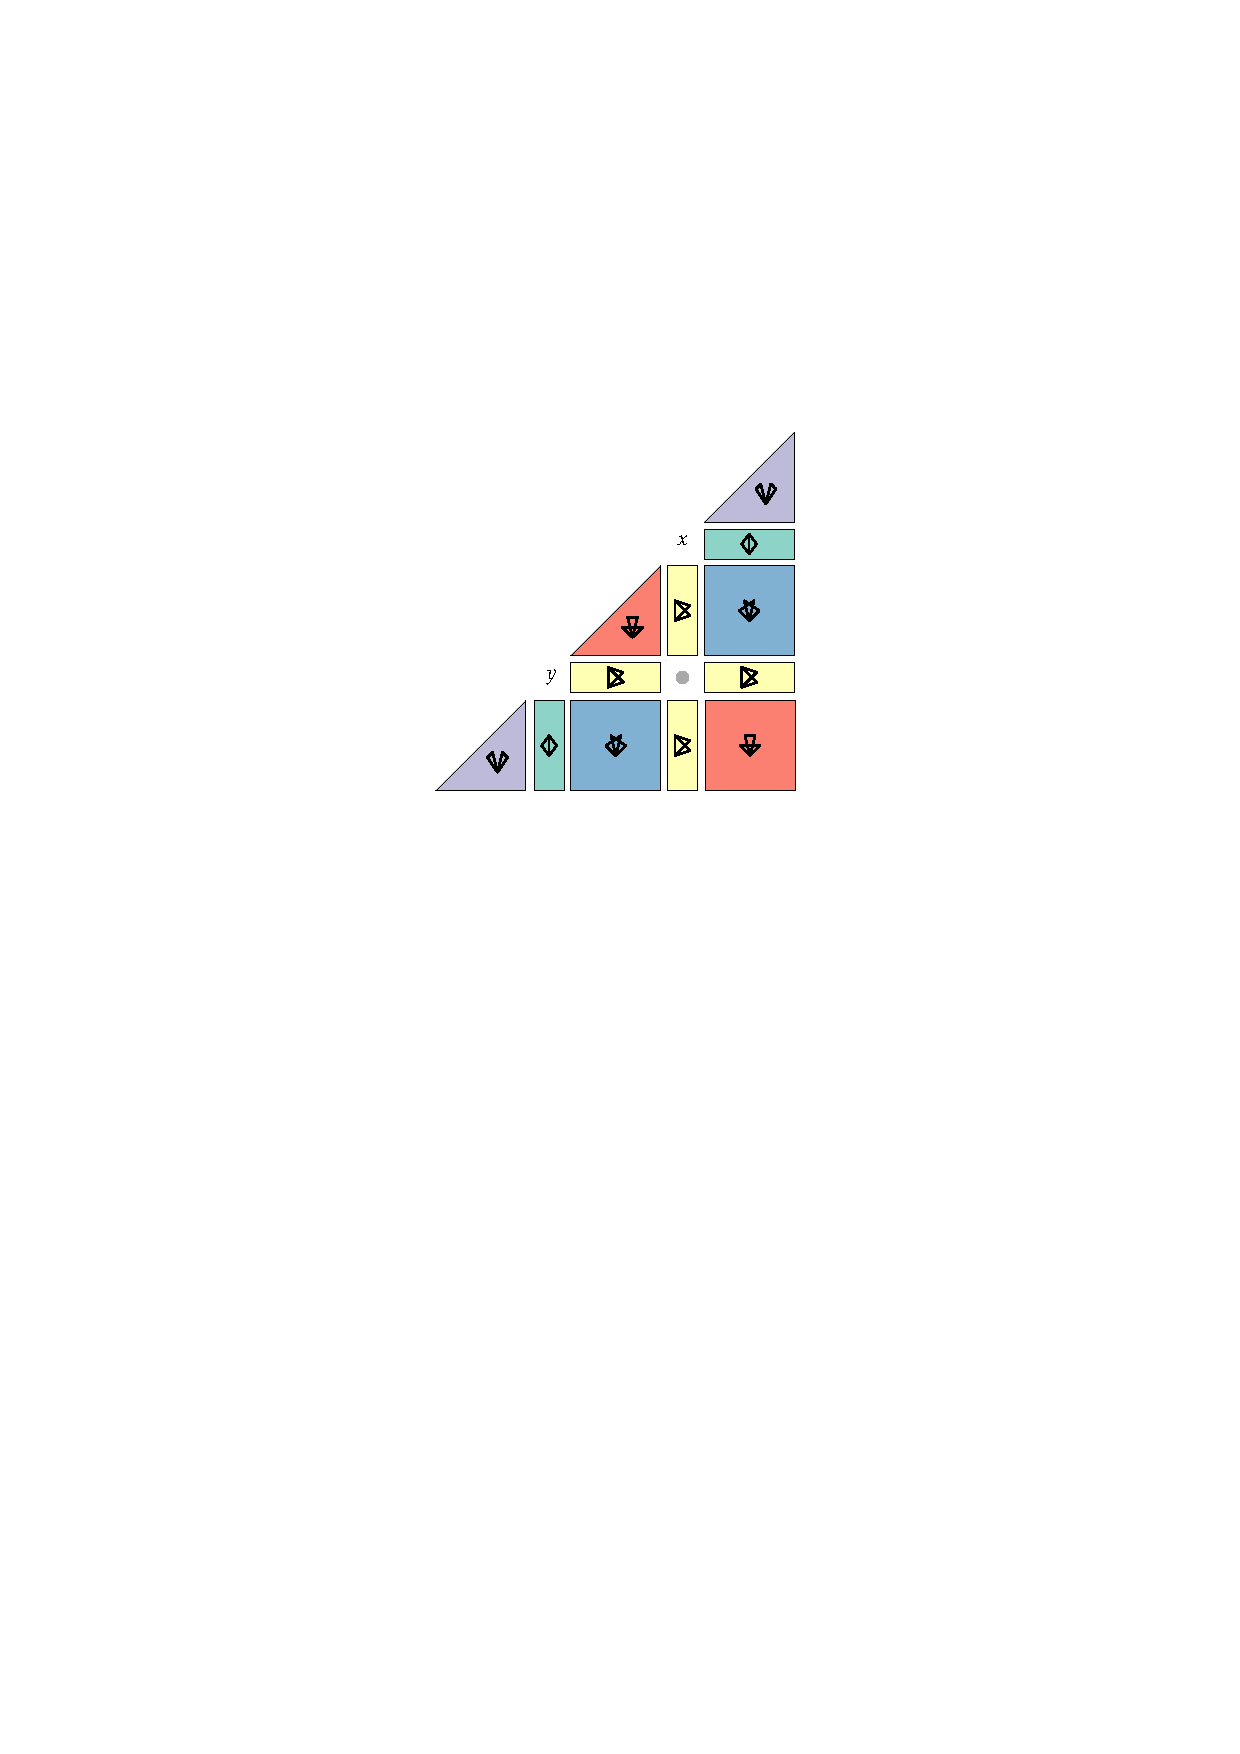
\includegraphics[width=.48\ka]{figs/crapper-2} & 
        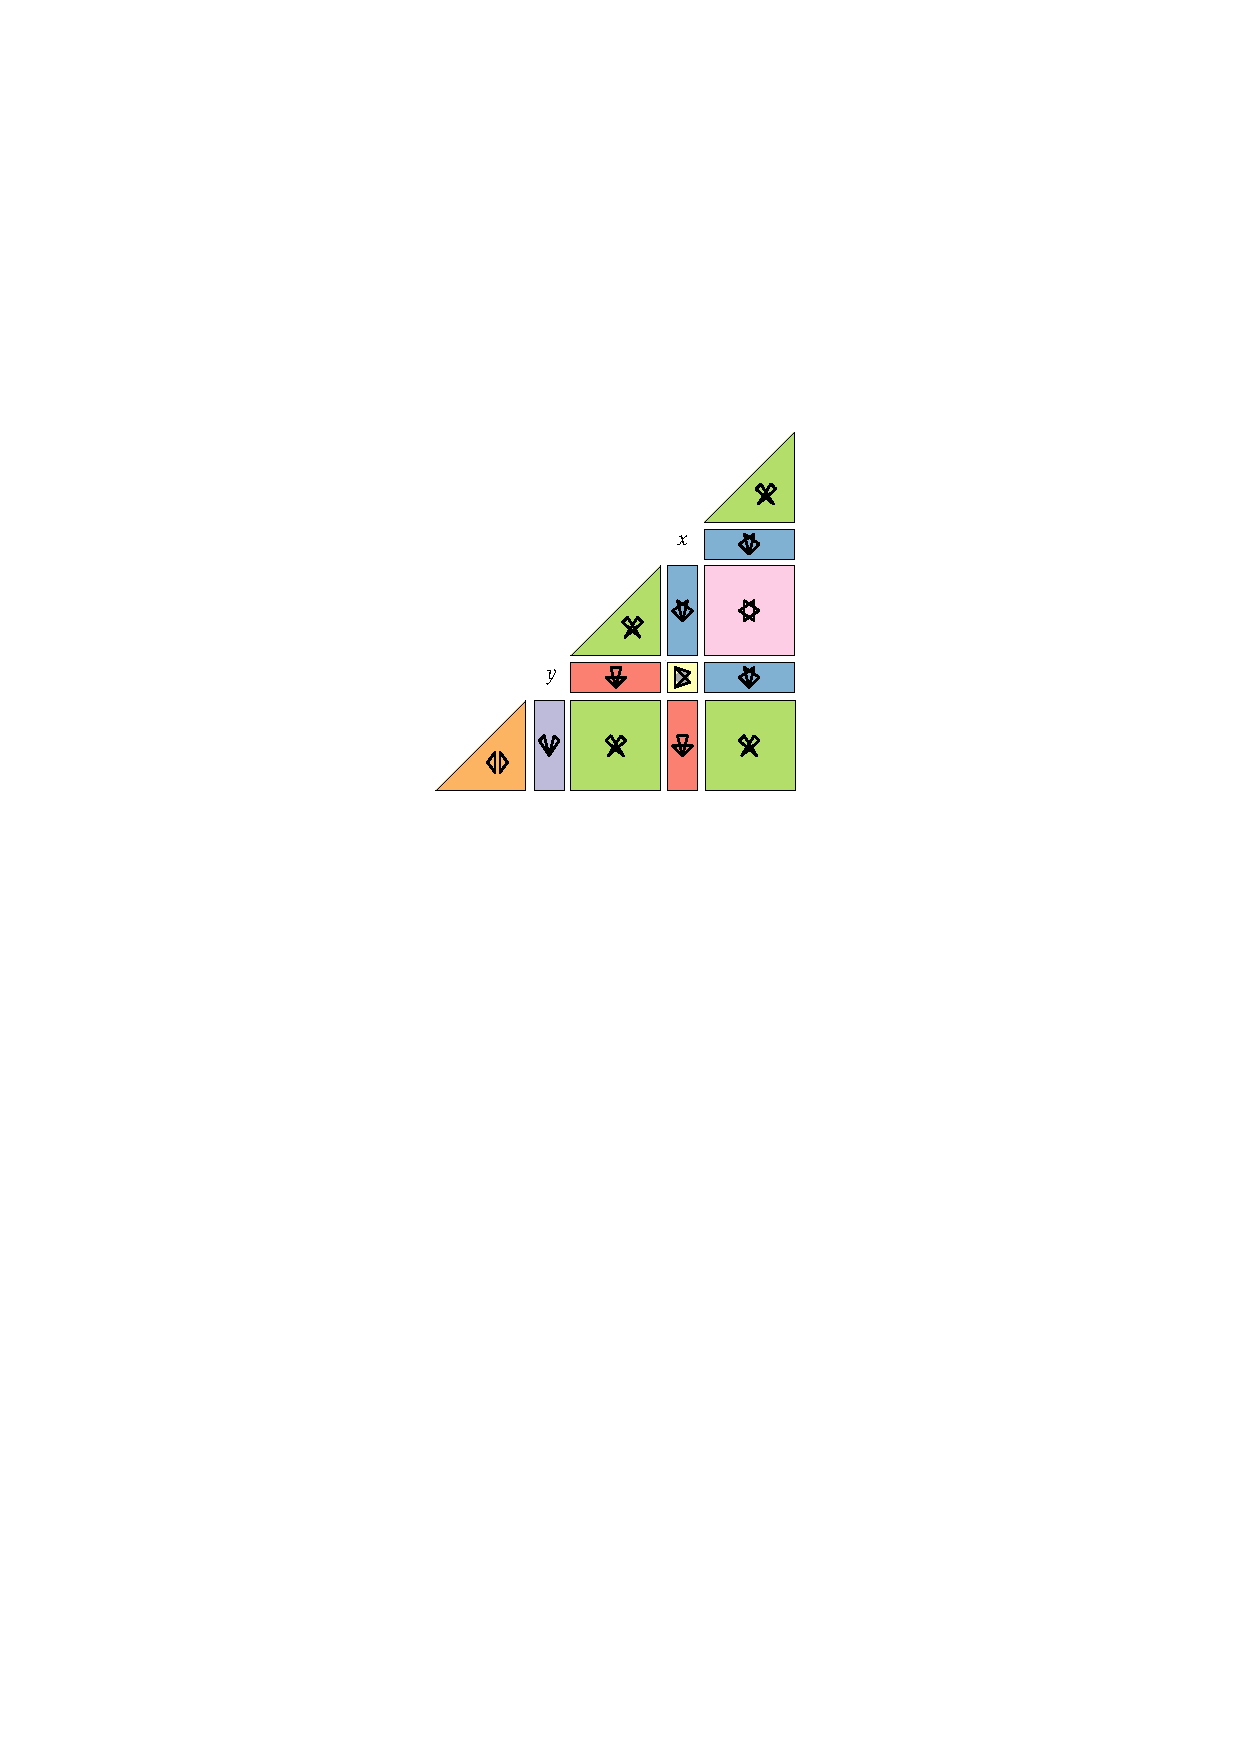
\includegraphics[width=.48\ka]{figs/crapper-1} 
      \end{tabular}
   }
   \centerline{
      \only<1>{\includegraphics{slidefigs/swords-region-1}}%
      \only<2>{\includegraphics{slidefigs/swords-region-2}}%
      \only<3>{\includegraphics{slidefigs/swords-region-3}}%
      \only<4->{\includegraphics{slidefigs/swords-region-4}}%
   }
   \uncover<4->{\hfill{QED}}\\
   \uncover<5->{$\ex'(n,\{\swords,\nested\})=O(n)$ and 
                $\ex'(n,\{\swords,\crossing\})=O(n)$ have similar proofs.}
\end{frame}



\begin{frame}
   \frametitle{$\ex'(n,\{\taco,\nested,\crossing\}) = O(n)$}
   \framesubtitle{
      %\newlength{\ka}
      \setlength{\ka}{.3\textwidth}
      \addtolength{\ka}{-1cm}
      \begin{tabular}{c@{\hspace{1cm}}c}
        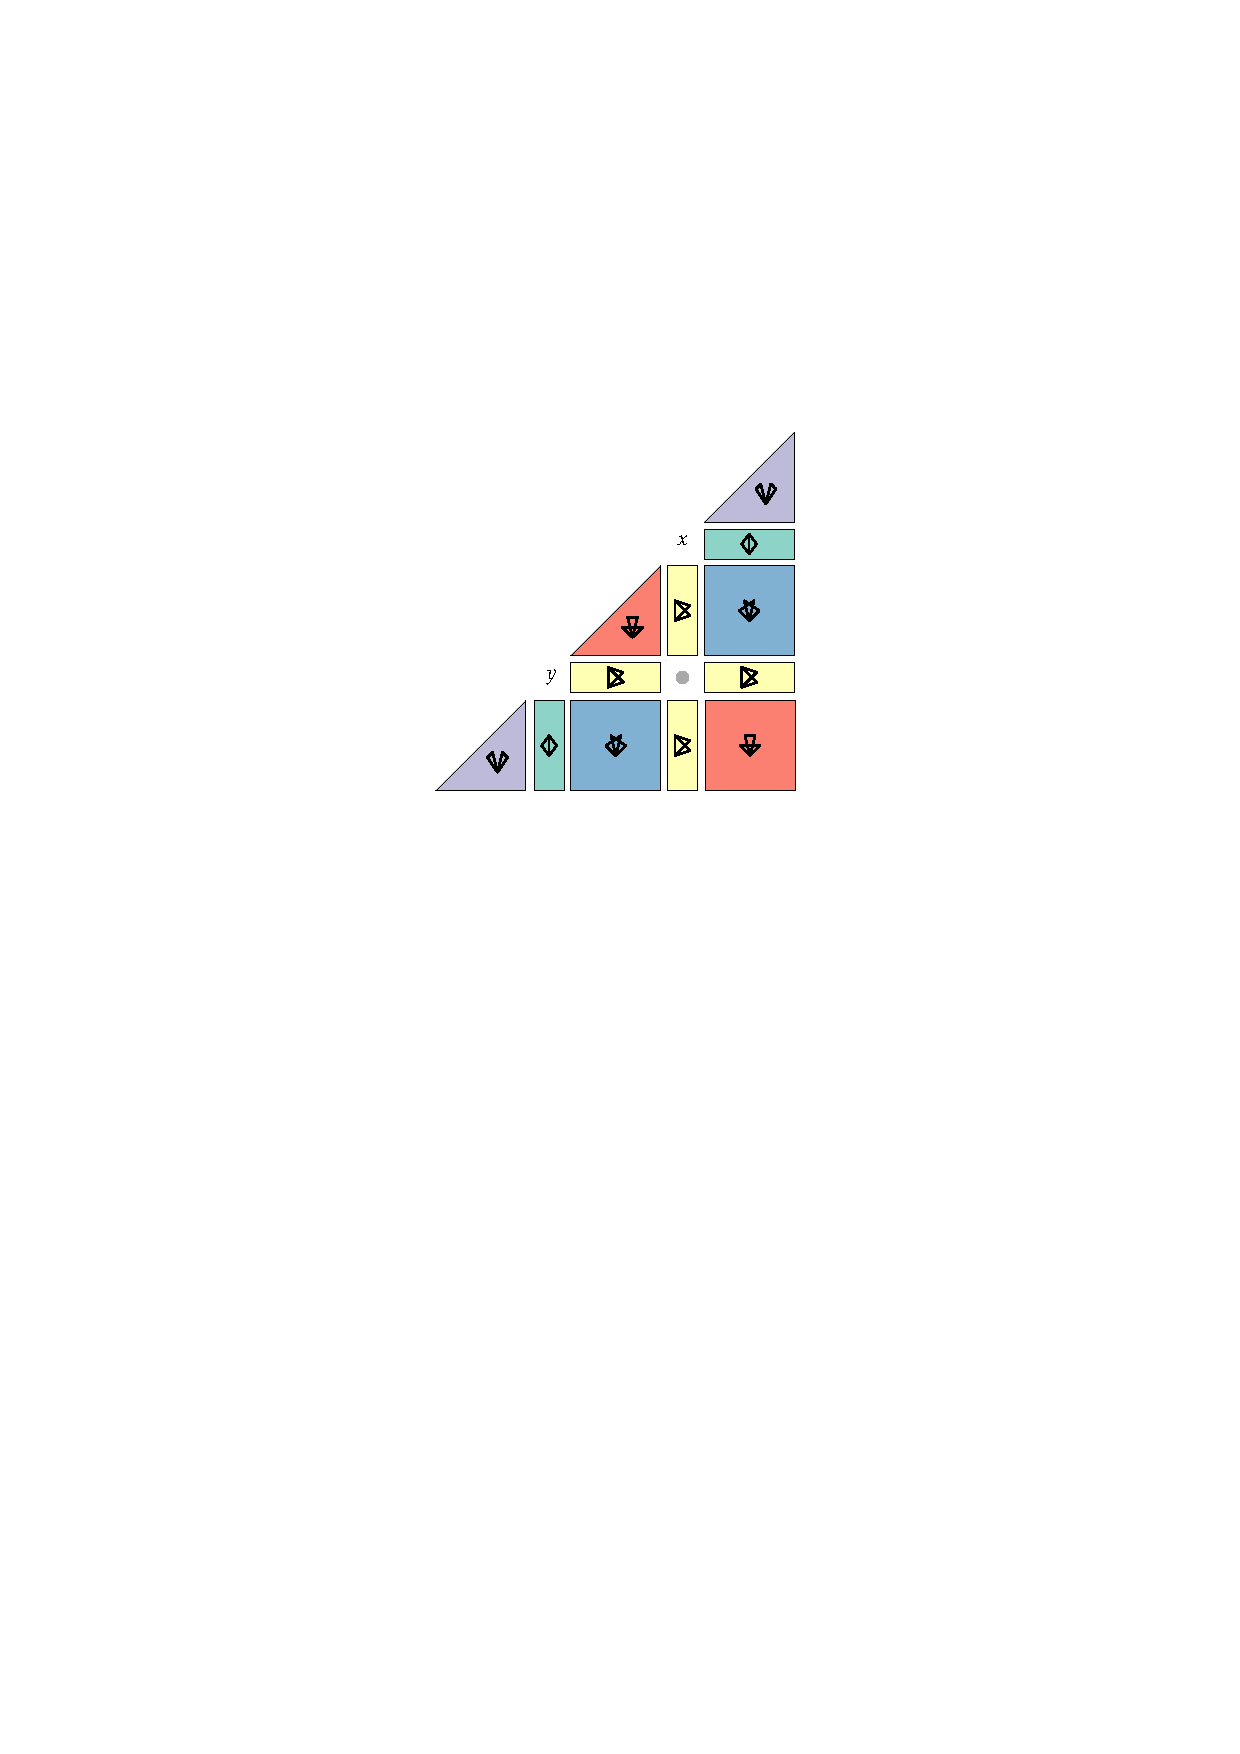
\includegraphics[width=.48\ka]{figs/crapper-2} & 
        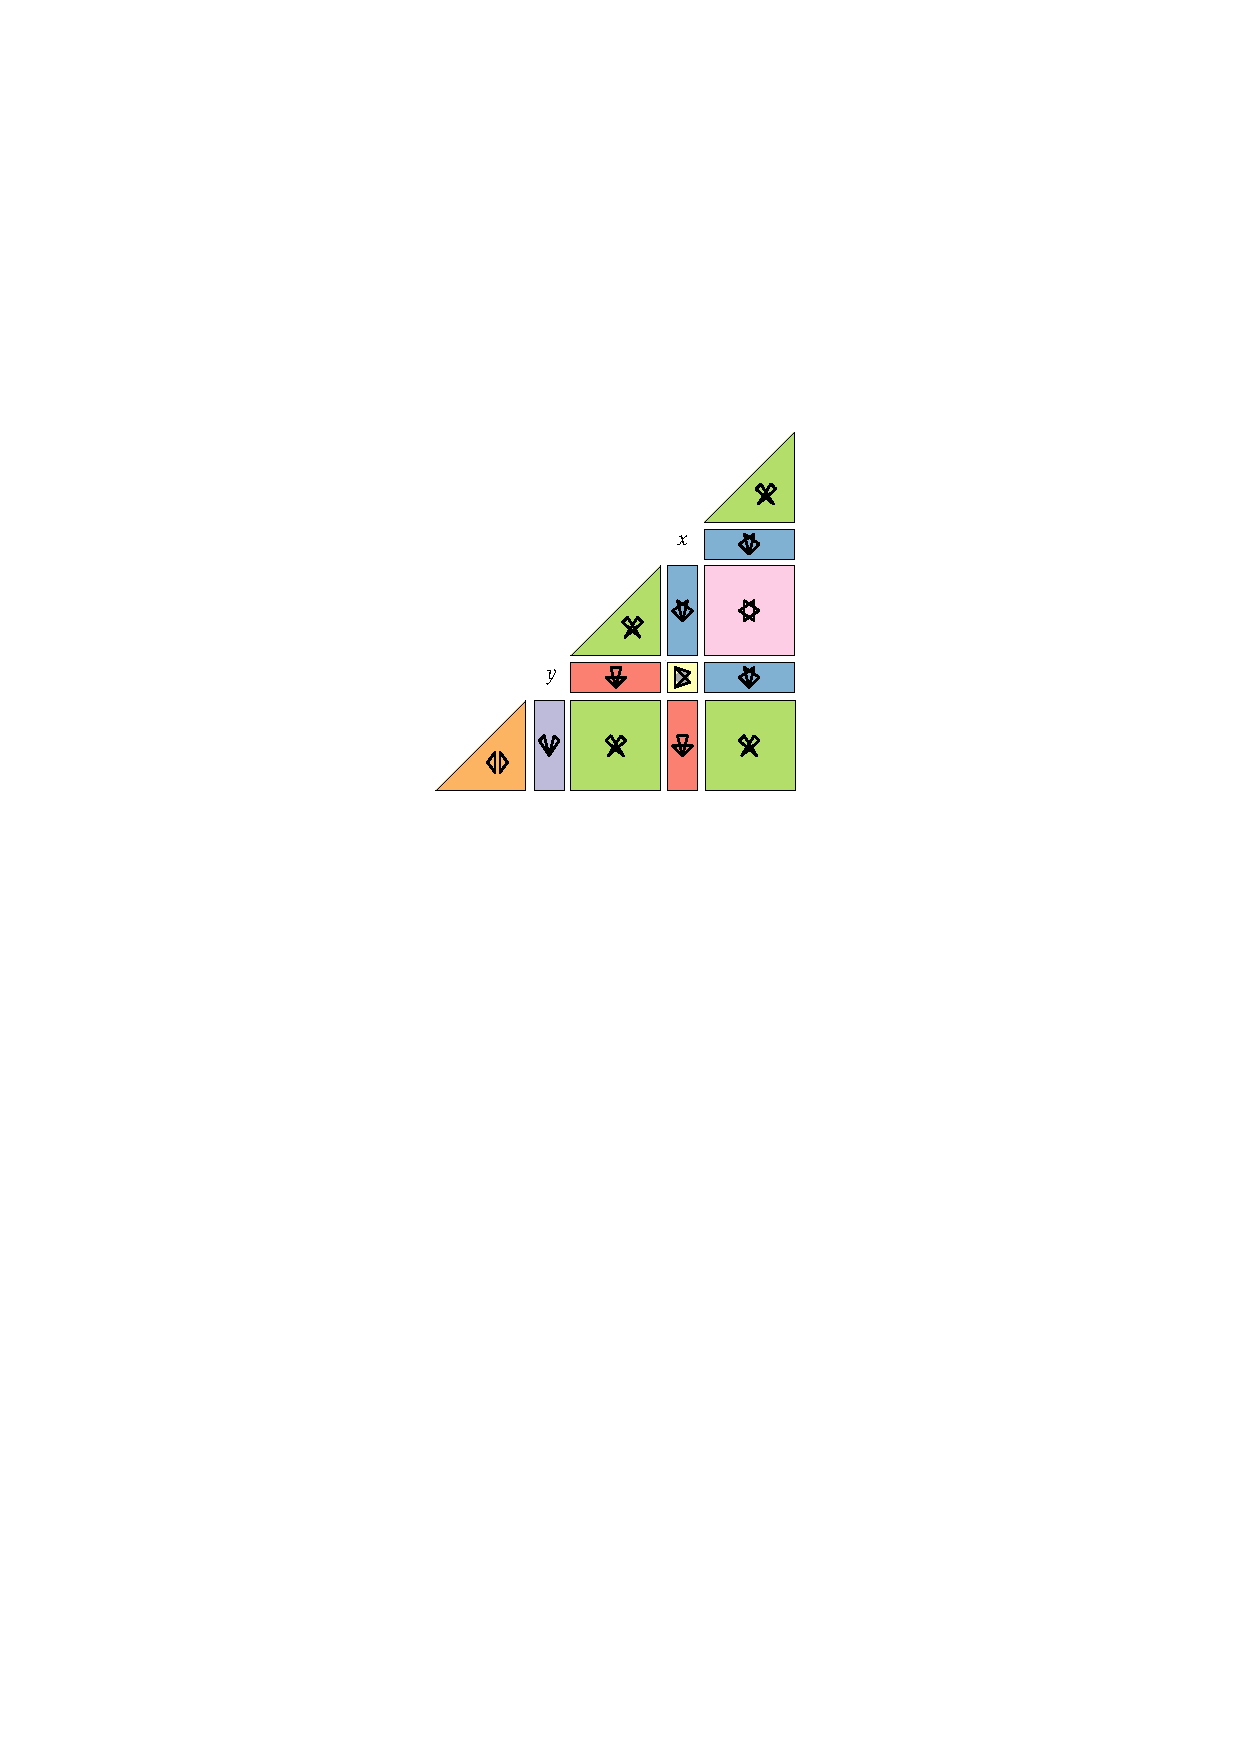
\includegraphics[width=.48\ka]{figs/crapper-1} 
      \end{tabular}
   }
   \begin{itemize}[<+->]
      \item \nested\ ensures points in one round are non-decreasing 
        \begin{itemize}
          \item Each point is in a new row or new column
        \end{itemize}
      \item Union of rules ensures these points are killed in subsequent rounds:\\[1ex]
         \centerline{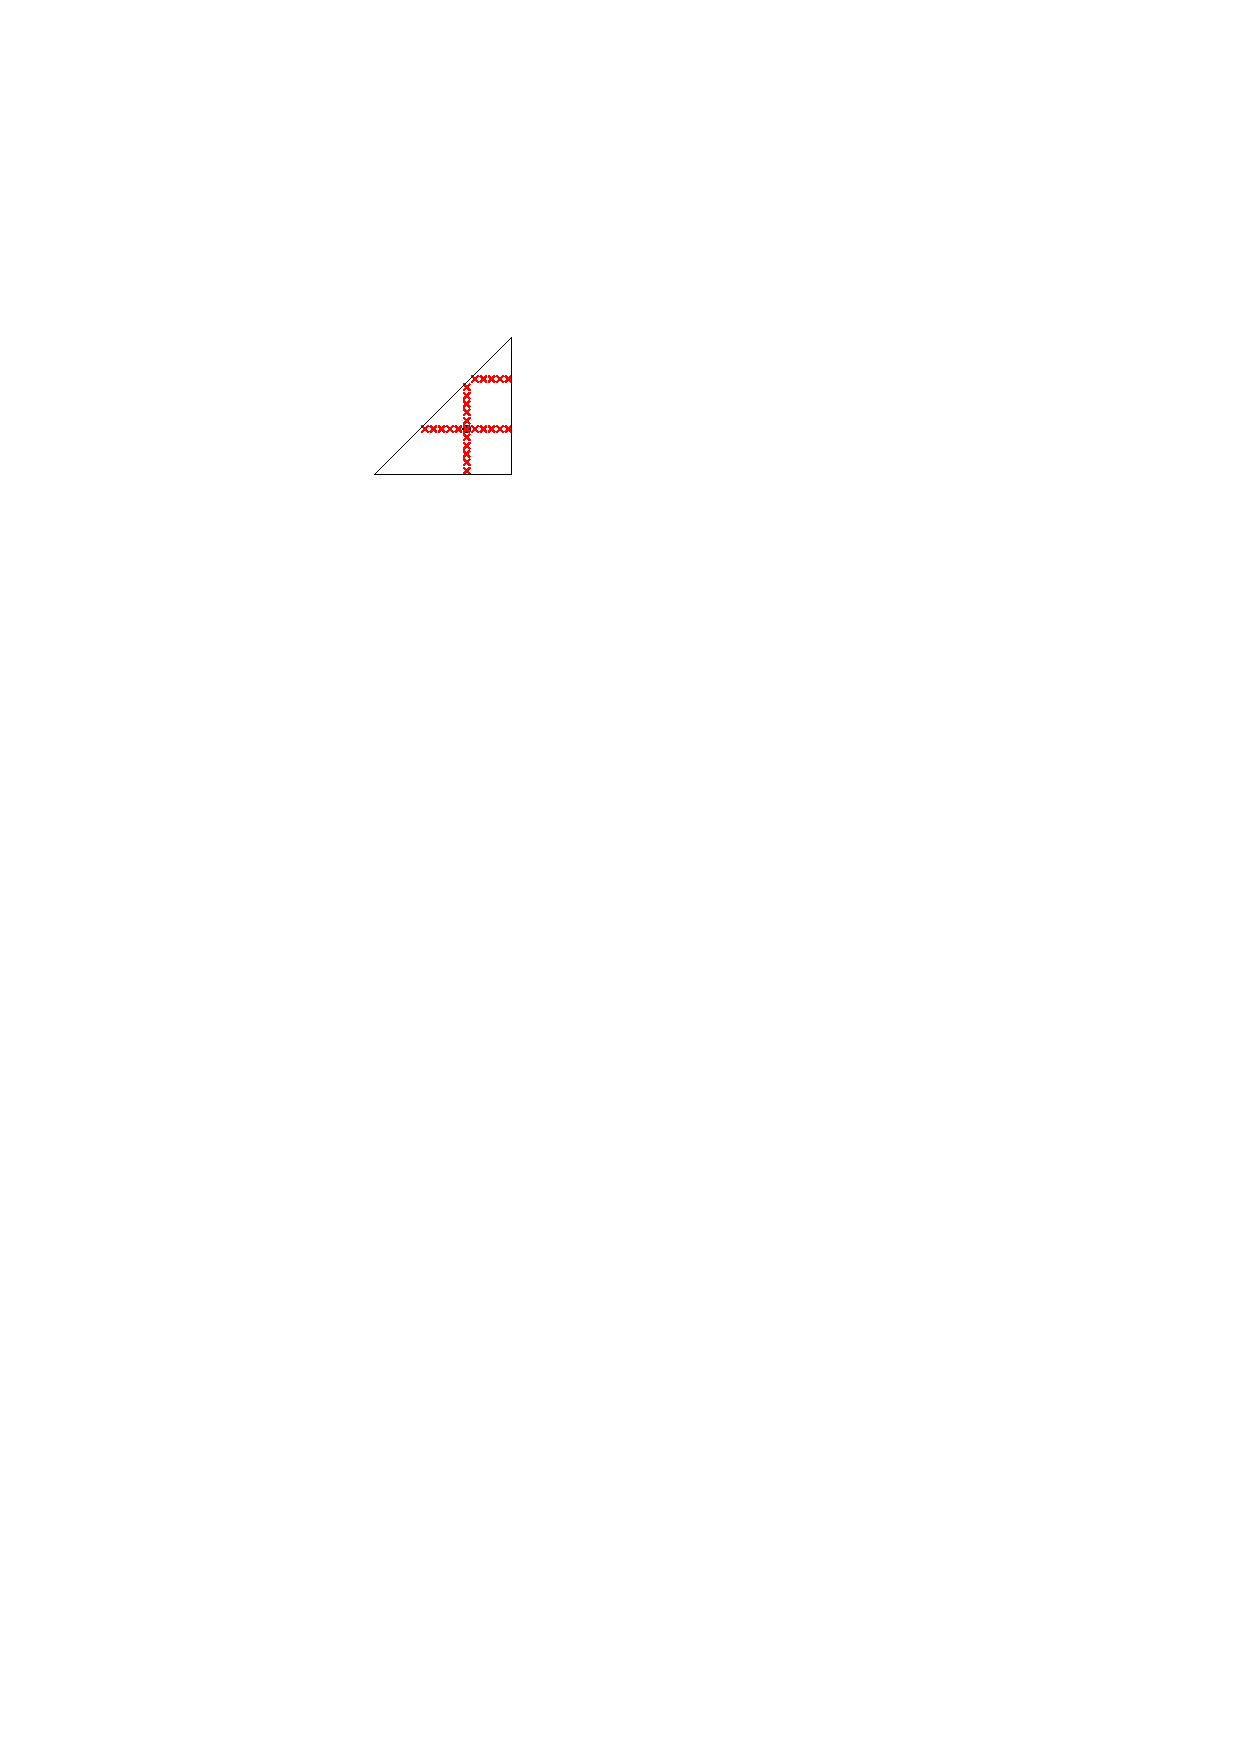
\includegraphics{figs/killers-10}}
      \item Each point in round $i$ kills one row or column in subsequent rounds\hfill{QED}
   \end{itemize}
\end{frame} 

\begin{frame}
   \frametitle{$\ex'(n,\{\taco,\nested\}) = O(n)$}
   \framesubtitle{
      %\newlength{\ka}
      \setlength{\ka}{.3\textwidth}
      \addtolength{\ka}{-1cm}
      \begin{tabular}{c@{\hspace{1cm}}c}
        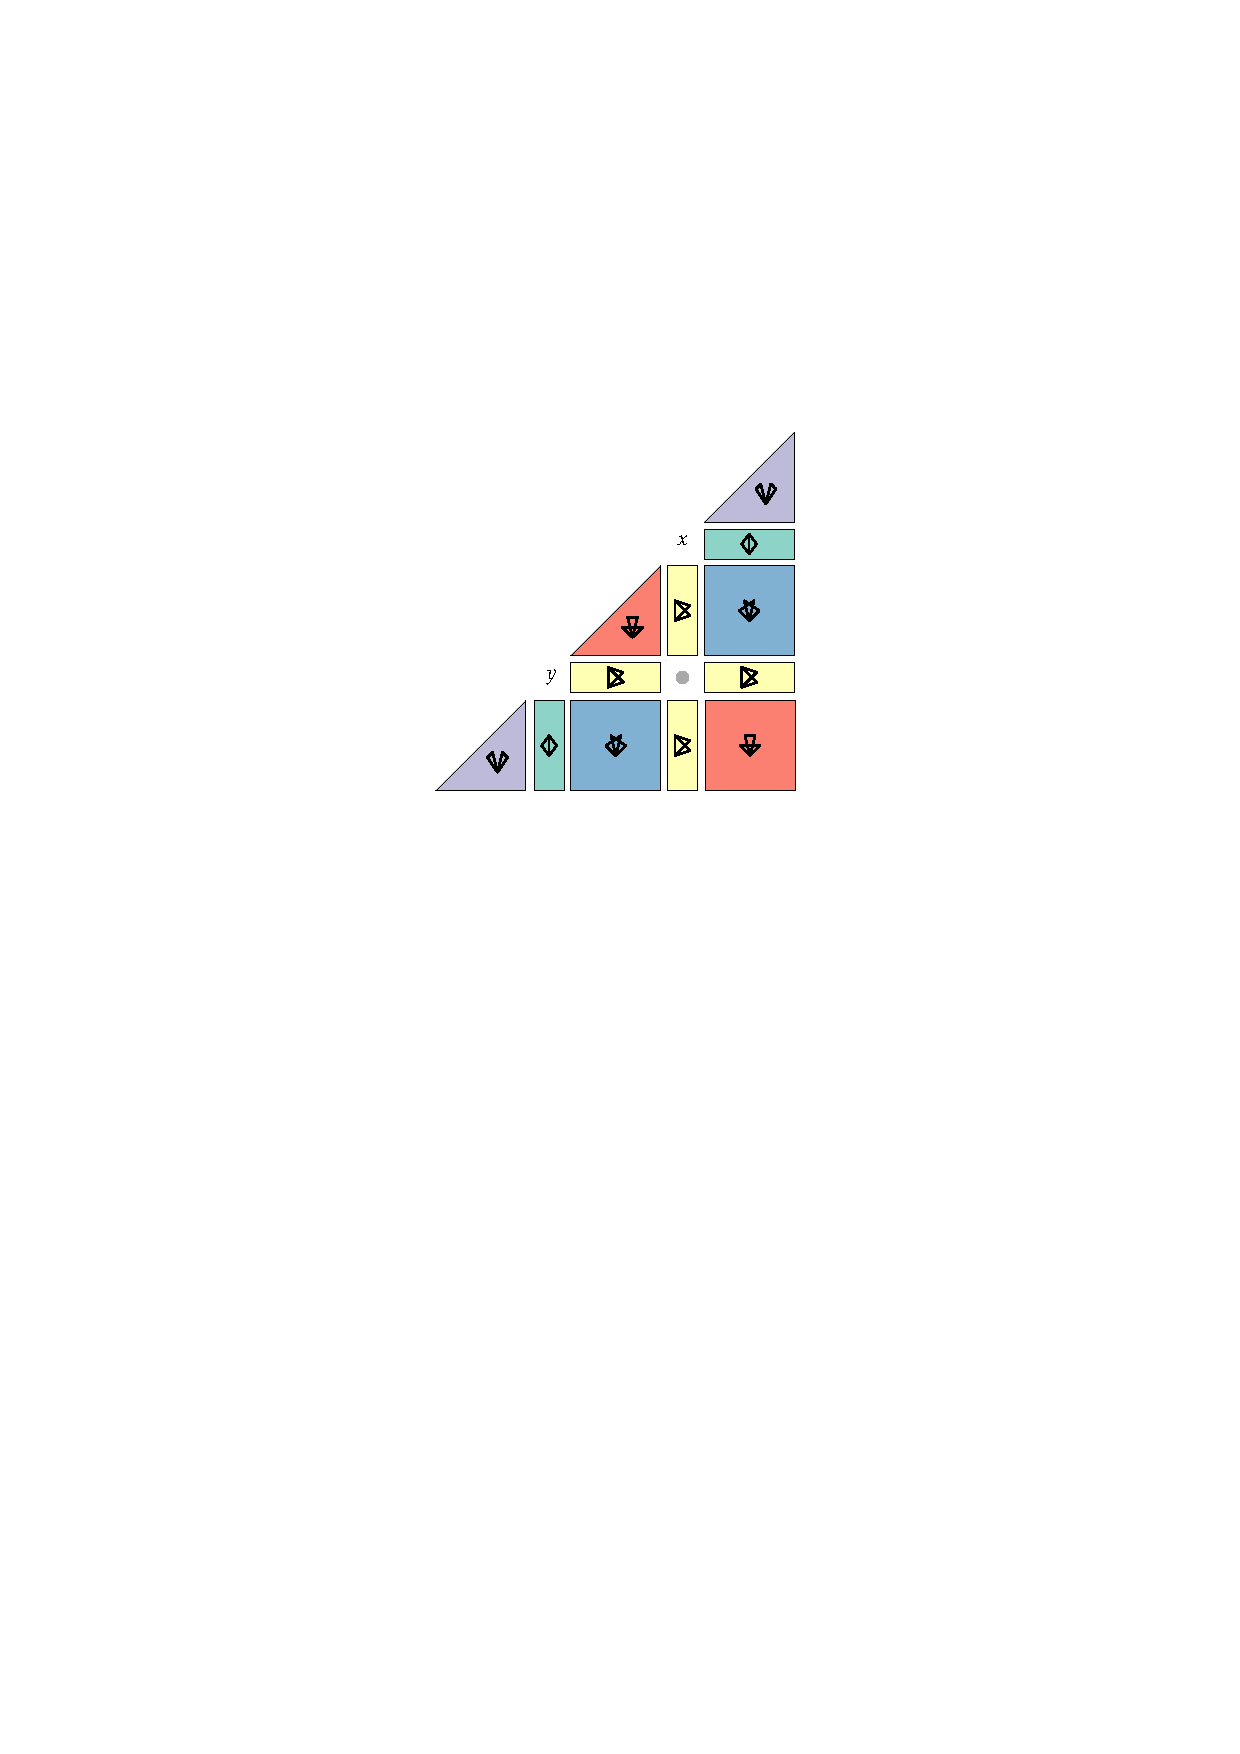
\includegraphics[width=.48\ka]{figs/crapper-2} & 
        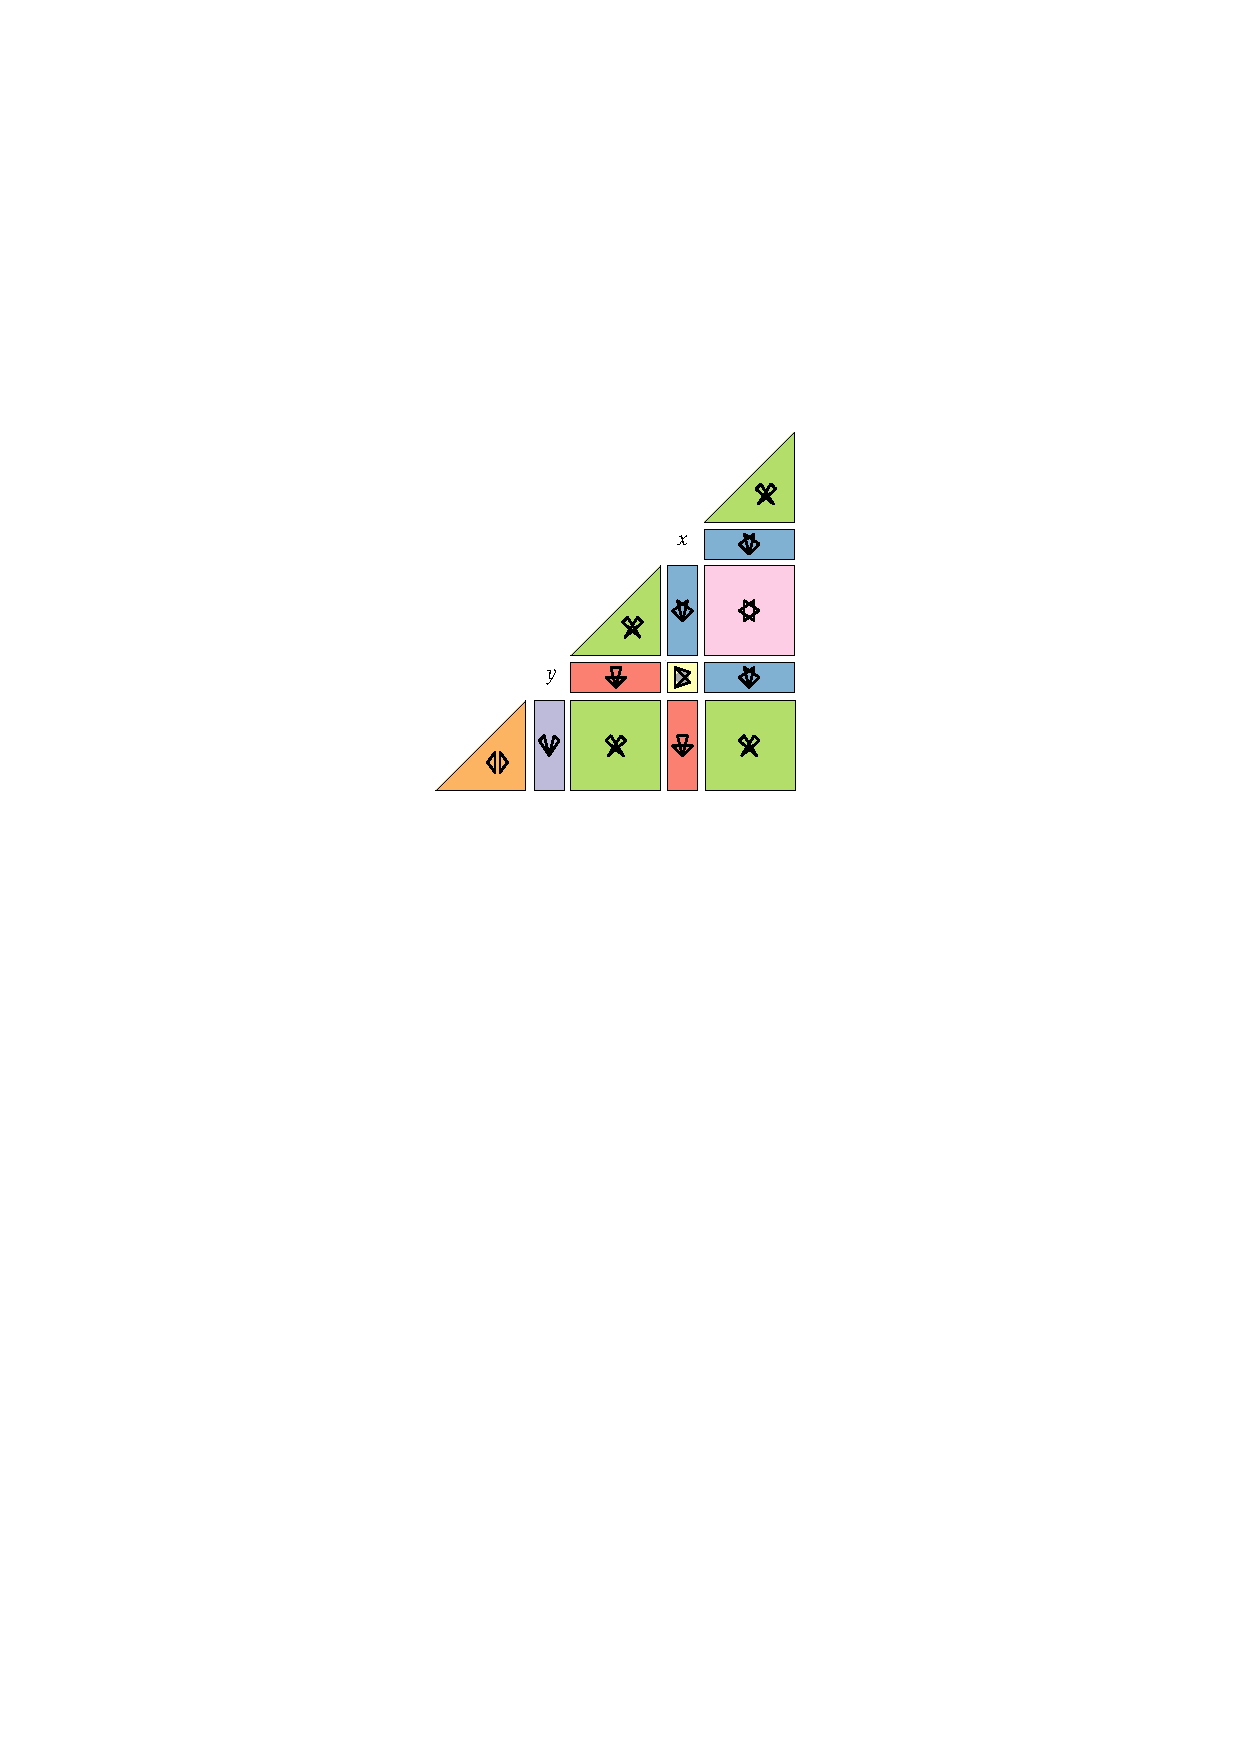
\includegraphics[width=.48\ka]{figs/crapper-1} 
      \end{tabular}
   }
   \begin{itemize}[<+->]
      \item Using these tools we have determined $\ex'(n,X)$ for any
        two element set $X$ \emph{except} $X=\{\taco,\nested\}$.
      \item The rules for $\ex'(n,X)$ for $\ex'(n,\{\taco,\nested\}$ give our
        dot-puzzle game.
      \item Did Bra\ss\ know this already in 2004?
   \end{itemize}
   
\end{frame}


\begin{frame}
   \frametitle{The End}
   \begin{center}
      %\newlength{\ka}
      \setlength{\ka}{.6\textwidth}
      \addtolength{\ka}{-1cm}
      \begin{tabular}{c@{\hspace{1cm}}c}
        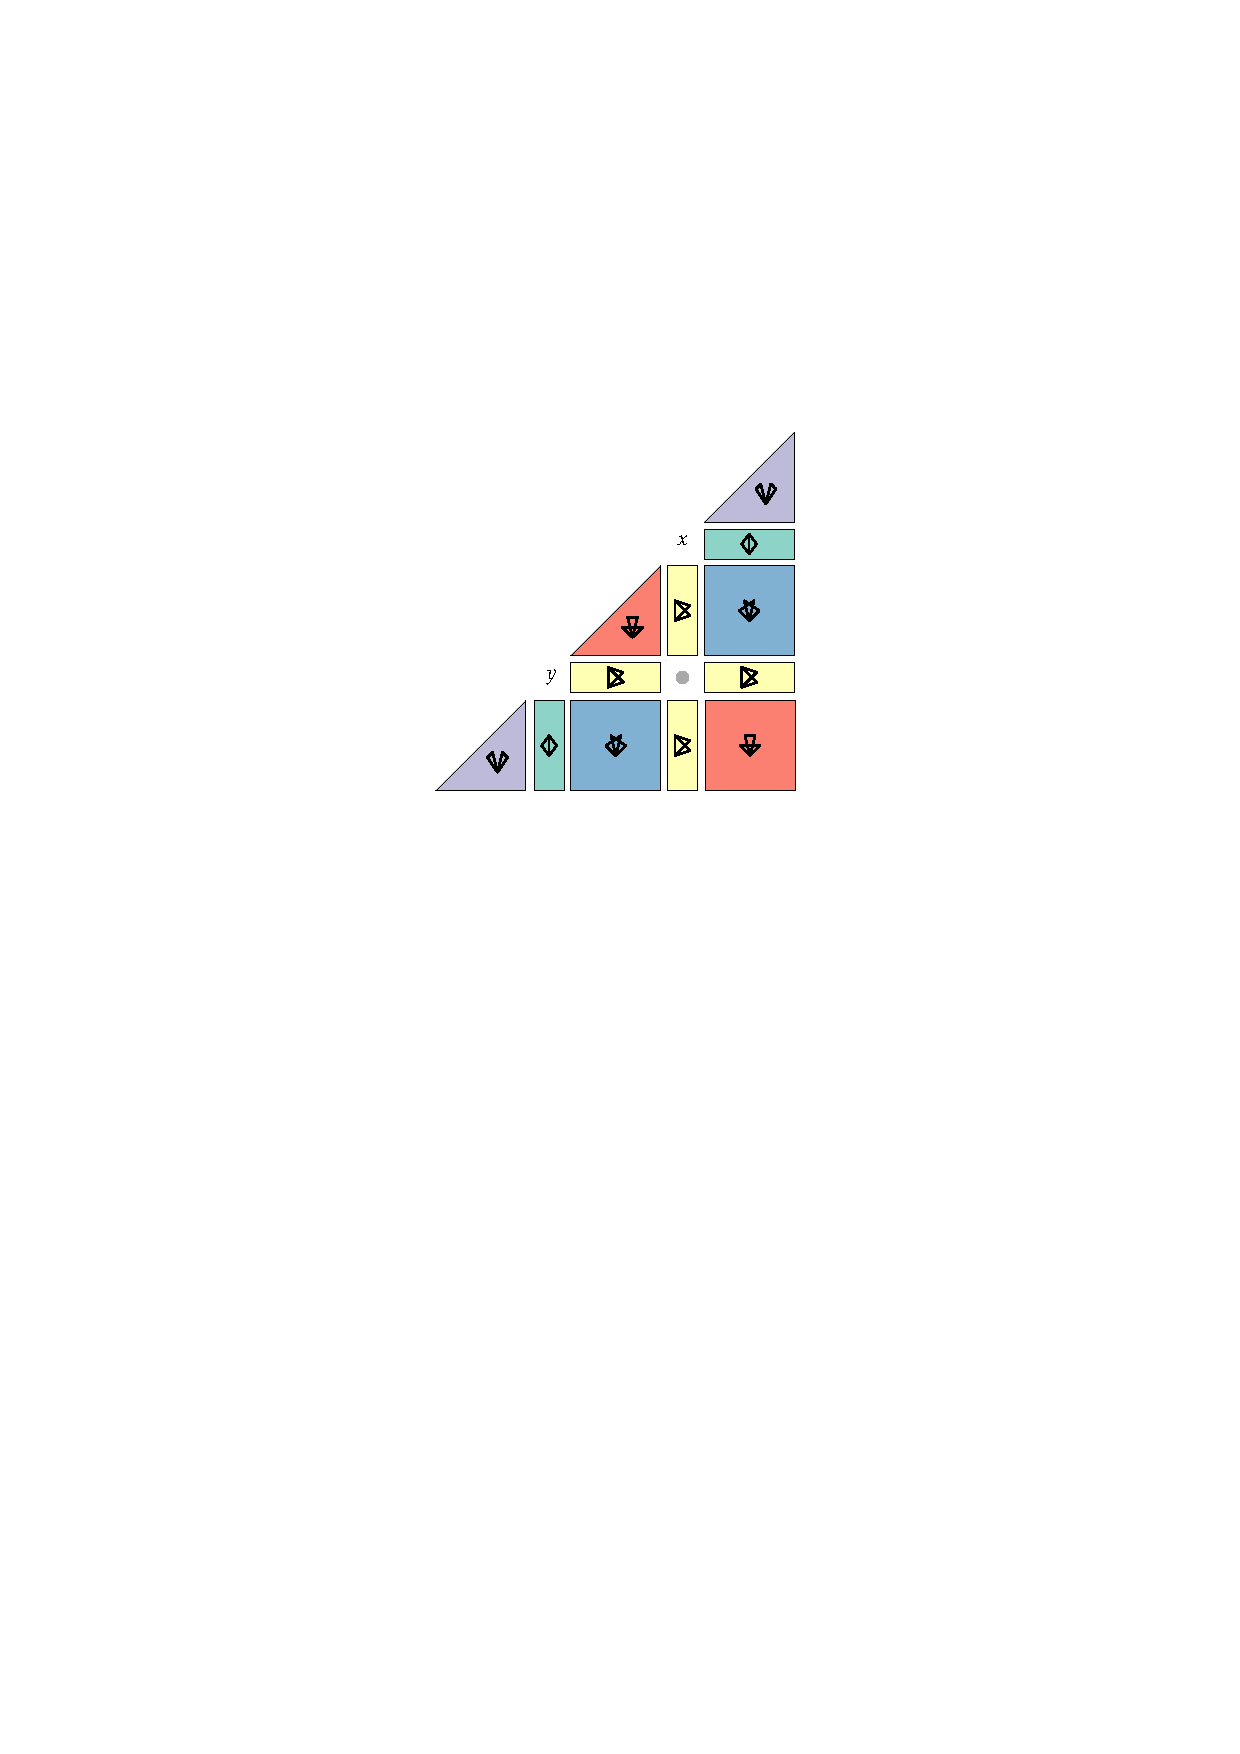
\includegraphics[width=.48\ka]{figs/crapper-2} & 
        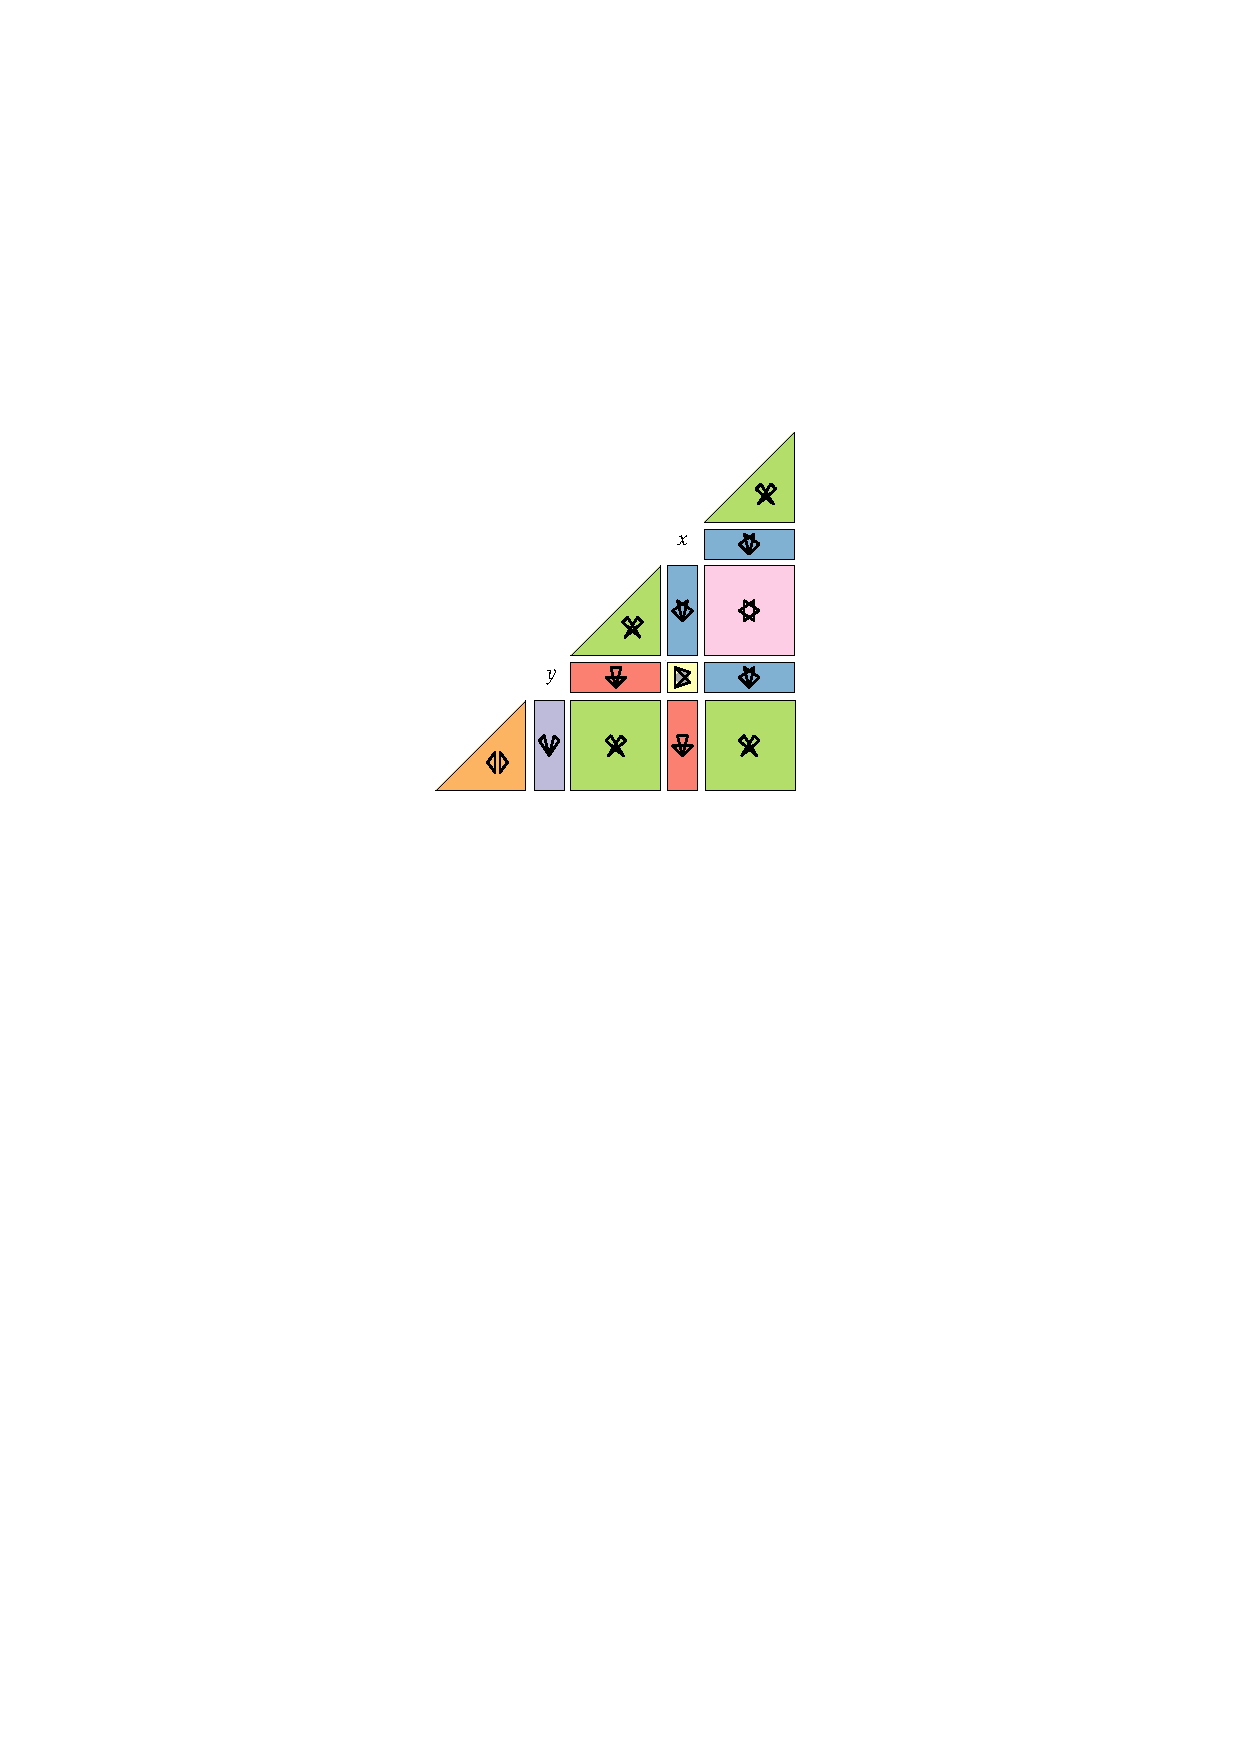
\includegraphics[width=.48\ka]{figs/crapper-1} 
      \end{tabular}
   \end{center}
   \centerline{\Huge Thanks!}
\end{frame}


\begin{frame}
   \frametitle{References}
   \begin{itemize}
      \item P. Braß. Tur\'an-type extremal problems for convex geometric
      hypergraphs. Contemporary Mathematics, \textbf{342}:25–34, 2004.
      
      \item P. Braß, G. Rote, and K. J. Swanepoel. Triangles of extremal area
      or perimeter in a finite planar point set. Discrete \& Computational
      Geometry, \textbf{26}(1):51–58, 2001.
      
      \item P. Erd\H{o}s and G. Purdy, Some extremal problems in geometry,
      Journal of Combinatorial Theory Series A, \textbf{10}:246–252, 1971.
   \end{itemize}
\end{frame}
 
\end{document}

